% ULaTeX2e, calling the article.cls class and 12-point type.

\documentclass[12pt]{article}

% My packages

\usepackage{framed, color}
\usepackage{soul}
\definecolor{blu}{rgb}{0,0,1}
\newcommand{\td}[1]{{\color{blu}\hl{TODO: #1}}}
\usepackage{graphicx}
\usepackage{amsthm}
\newtheorem{mydef}{Definition}
\usepackage{dcolumn}
\usepackage{multirow}
\usepackage{booktabs}
\newcolumntype{d}{D{.}{.}{4.0}}
\newcolumntype{s}{D{.}{.}{1.4}}

% Users of the {thebibliography} environment or BibTeX should use the
% scicite.sty package, downloadable from *Science* at
% www.sciencemag.org/about/authors/prep/TeX_help/ .
% This package should properly format in-text
% reference calls and reference-list numbers.

\usepackage{scicite}

% Use times if you have the font installed; otherwise, comment out the
% following line.

\usepackage{times}

% The preamble here sets up a lot of new/revised commands and
% environments.  It's annoying, but please do *not* try to strip these
% out into a separate .sty file (which could lead to the loss of some
% information when we convert the file to other formats).  Instead, keep
% them in the preamble of your main LaTeX source file.


% The following parameters seem to provide a reasonable page setup.

\topmargin 0.0cm
\oddsidemargin 0.2cm
\textwidth 16cm 
\textheight 21cm
\footskip 1.0cm


%The next command sets up an environment for the abstract to your paper.

\newenvironment{sciabstract}{%
\begin{quote} \bf}
{\end{quote}}


% If your reference list includes text notes as well as references,
% include the following line; otherwise, comment it out.

\renewcommand\refname{References and Notes}

% The following lines set up an environment for the last note in the
% reference list, which commonly includes acknowledgments of funding,
% help, etc.  It's intended for users of BibTeX or the {thebibliography}
% environment.  Users who are hand-coding their references at the end
% using a list environment such as {enumerate} can simply add another
% item at the end, and it will be numbered automatically.

\newcounter{lastnote}
\newenvironment{scilastnote}{%
\setcounter{lastnote}{\value{enumiv}}%
\addtocounter{lastnote}{+1}%
\begin{list}%
{\arabic{lastnote}.}
{\setlength{\leftmargin}{.22in}}
{\setlength{\labelsep}{.5em}}}
{\end{list}}


% Include your paper's title here

\title{Hysteresis in human computation:\\ how one task affects another} 


% Place the author information here.  Please hand-code the contact
% information and notecalls; do *not* use \footnote commands.  Let the
% author contact information appear immediately below the author names
% as shown.  We would also prefer that you don't change the type-size
% settings shown here.

\author
{Edward Newell, Derek Ruths,\\
\\
\normalsize{\texttt{edward.newell@mail.mcgill.ca}}\\
\normalsize{\texttt{druths@networkdynamics.org}}\\
\normalsize{School of computer science, McGill University,}\\
\normalsize{3630 rue University, Montreal, Quebec, H3A 0C6, Canada}\\
\\
}

% Include the date command, but leave its argument blank.

\date{}



%%%%%%%%%%%%%%%%% END OF PREAMBLE %%%%%%%%%%%%%%%%



\begin{document} 

% Double-space the manuscript.

\baselineskip24pt

% Make the title.

\maketitle 



% Place your abstract within the special {sciabstract} environment.

\begin{sciabstract}

Faced with the scale and complexity of the data revolution, researchers and
industry are increasingly relying on \textit{human computation}.  Microtask
platforms, like Amazon Mechanical Turk, act like a human compute server,
making it possible to access human cognition quickly and inexpensively. 
This has lead to broad adoption across a spectrum of disciplines
in the humanities and computer science, as well as in research into medical 
imaging technologies and other applications where expert opinion would 
normally be sought.  Here we show that an inherent
feature of microtask platforms, the repetition of similar tasks,
acts as a strong, but as yet unexplored source of bias.  
These \textit{intertask effects} rival the
severity of overtly framing a task's purpose.  
Using image-labeling as a canonical microtask, we found that prior 
tasks influence the vocabulary that a worker uses when labeling 
subsequent images in both profound an nuanced ways.  Prior tasks not only 
alter what a worker focuses on, 
but also modulate the richness and specialization of her vocabulary.  
While intertask effects can be a source of systematic bias, our
results suggest that, when properly controlled, they can be leveraged
to hone worker focus and specificity.  Though we focused on microtask 
platforms due to their emerging prominence, our results apply to  
citizen science, crowdsourcing, and any application involving repetitive 
tasks relying on human judgment.
\end{sciabstract}

\section*{Introduction}
Microtask platforms are online marketplaces on which \textit{requesters} 
post batches of tasks, and \textit{workers} complete them
for remuneration, a sense of purpose, and for fun
\cite{kazai2013analysis,Antin20122925}.  
Typical tasks include tagging and categorizing images 
\cite{6116320,Zhai2012357}, transcribing voice recordings 
\cite{chandler2013breaking,paolacci2010running}
or handwritten notes \cite{Berinsky2012351,Finnerty2013}, and judging the 
relevancy of search results 
\cite{le2010ensuring,grady2010crowdsourcing,alonso2009can,kazai2013analysis}.

While microtask platforms have been widely adopted as a research tool,
computer scientists also hold such platforms as the object of 
research, viewing  microtask platforms as a new kind of computing 
architecture.  In analogy to CPUs (central 
processing units) and GPUs (graphics processing units), 
Davis \textit{et al} invoked the \textit{human processing unit}, or HPU \cite{5543192}.
Meanwhile, researchers have sought to define a basic HPU instruction set, and
libraries for HPU programming are under active development
 \cite{little2010turkit,minder2011crowdlang,minder2012crowdlang,kittur2011crowdforge}.  

Unlike CPUs and GPUs, the experiments we present here suggest HPUs
are subject to \textit{hysteresis}, meaning that their outputs depend
on the history of their inputs.  Given the
increasing prevalence of microtask-based research methods, other factors 
affecting HPU outputs have received considerable attention.
This includes various task-design parameters such as the level of 
pay \cite{kazai2013analysis}, the training \cite{le2010ensuring} and 
pre-screening \cite{paolacci2010running} of workers, and user-interface 
design factors \cite{Finnerty2013}.  
Researchers have also investigated \textit{framing} effects, 
such as the effects of describing the workflow context 
\cite{Kinnaird2012281}, the purpose of tasks 
\cite{chandler2013breaking}, or altering the problem description
\cite{thibodeau2013natural}.  Results in psychology show that people are 
susceptible to various kinds of priming 
\cite{BJOP1796,No2007,beller1971priming}, and, in particular, 
task-repetition effects \cite{Gass1999549,sohn2001task}.  But to our 
knowledge, no study has investigated the practical ramifications 
of intertask effects on human computation.

We investigated intertask effects using image-labeling tasks on the Amazon 
Mechanical Turk (MTurk) microtask platform.  Image-labeling tasks are among
the most common MTurk tasks \cite{chandler2013breaking,Berinsky2012351,Finnerty2013,paolacci2010running}, a trend which will probably continue 
in the long term because of their role in computer vision research 
\cite{5543192}.
In our experiments, workers performed a set of \textit{initial tasks}, 
followed by a set of \textit{test tasks}. Crucially, no distinction was
made between these sets from the perspective of the worker. We varied the 
initial tasks (for example, having workers label images of food or objects), 
and observed the ensuing effects on responses in test tasks.  
As a point of 
comparison, we also included treatments in which we framed the tasks in terms 
of different purposes.

The results showed that intertask effects are stronger than framing effects.  
Framing effects were comparable to intertask effects only when the workers 
were asked to actively reiterate the frame by means of a combo-box input.
Using the wordnet corpus (\#), we found that intertask 
effects can hone a worker's focus, and boost the specialization
and lexical richness of her labels.  Thus, while intertask effects may be a 
serious source of bias, they can also be leveraged to help achieve
expert-level performance in crowdsourcing, when properly controlled.

\paragraph{Experimental setup.}
\begin{figure}
	\centering
	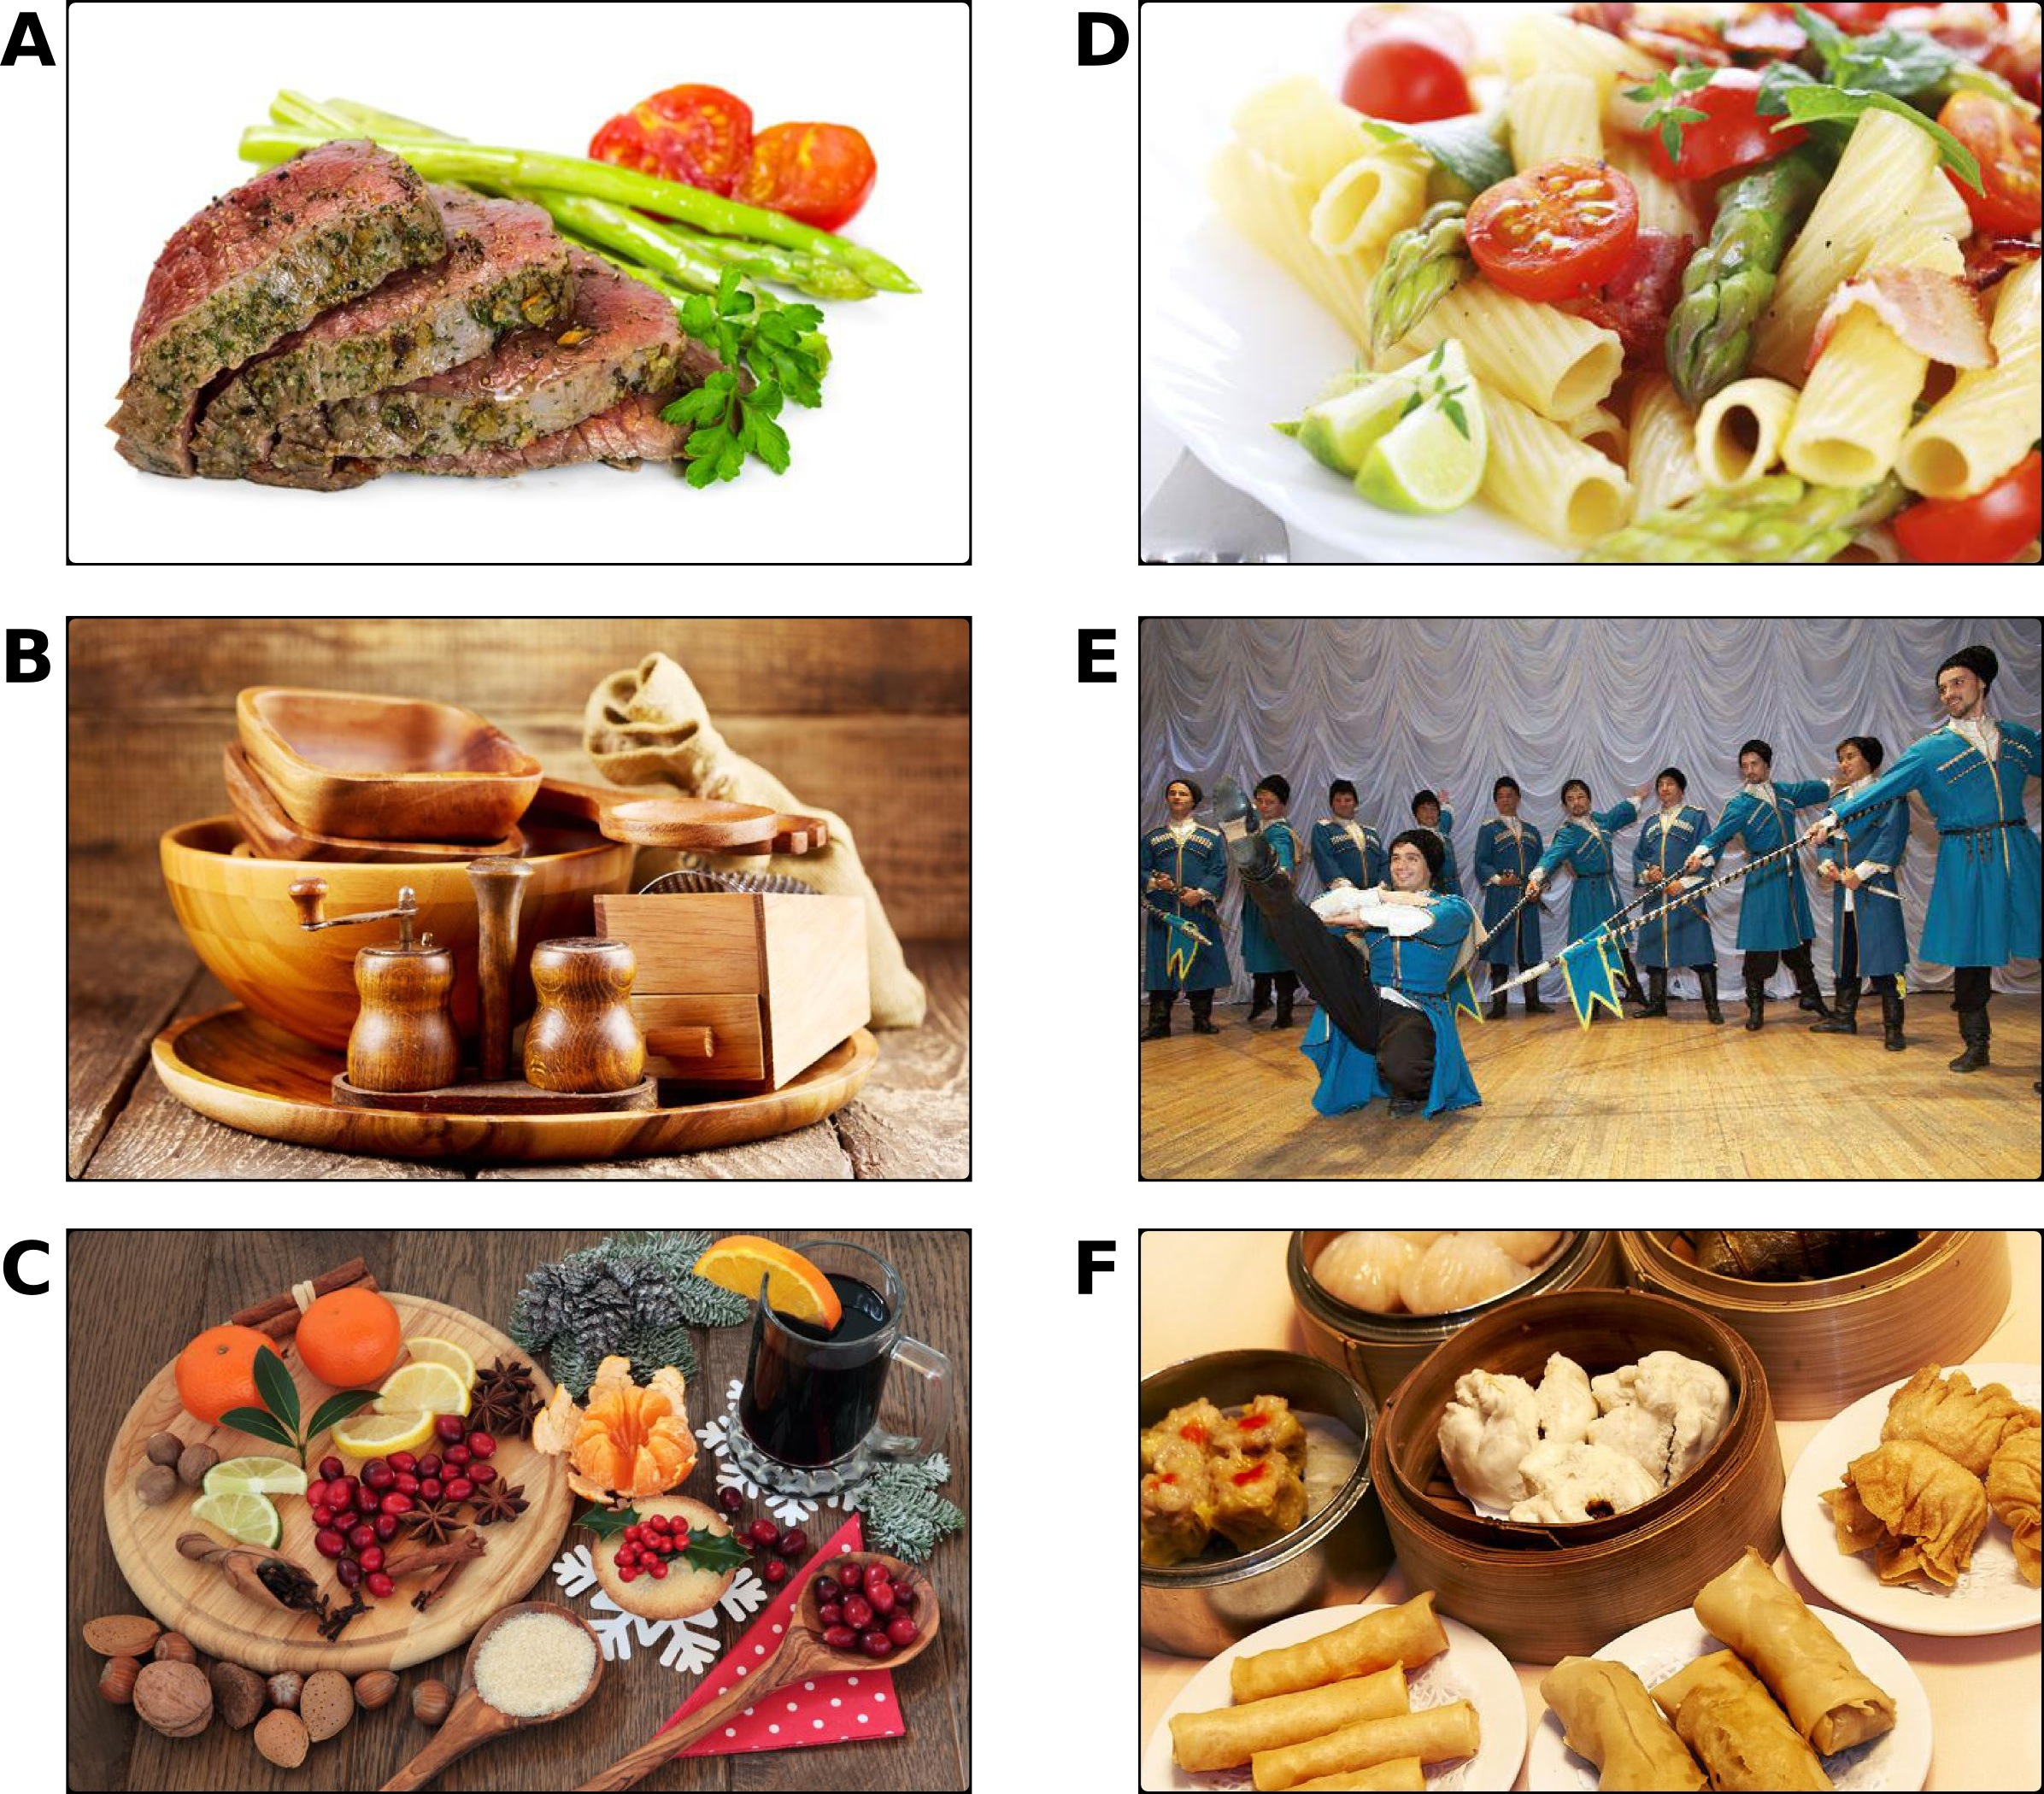
\includegraphics[scale=0.7]{figs/images.pdf}
	\caption{
		Examples of images used for various experiments and treatments:
		A) initial task for \textit{task1:food}, B) initial task for 
		\textit{task1:obj}, C) test task for treatments in \textit{exp1}, 
		D) initial task for \textit{task2:food}, 
		E) initial task for \textit{task2:cult},  
		F) test task for treatments in \textit{exp2}.  
		The full set of experimental materials is shown in the 
		supplementary text.
	}

	\label{fig:task}
\end{figure}

We performed two experiments, \textit{exp1} and \textit{exp2}, which consisted
of various pairs of treatments.  The treatments in each pair were subjected to
the same exposure modality, either initial tasks or framing, but differed in
the content of the exposure.  Table \ref{table:treatments}  
summarizes the treatments and introduces a naming convention that we use 
in what follows.
In \textit{exp1}, workers in the treatment pair \textit{task1} initially
labeled 5 images containing either food (treatment \textit{task1:food}), or 
objects (\textit{task1:obj}), and then performed test tasks, in 
which they 
labeled images containing both food and objects (see Fig.~\ref{fig:task} for 
examples of the images used). In \textit{exp1}, we included two other 
treatment pairs, \textit{frame1} and \textit{echo1}, in which workers did not 
perform initial tasks, but instead were given information which framed the 
purpose of the tasks.  Workers in \textit{frame1} were told that the tasks 
were ``Funded by the laboratory for the visual perception of 
\{ Food and Ingredients $\vert$ Objects and Tools~\}''.  In \textit{echo1},
we sharpened the frame, by indicating that ``The purpose of this study is to 
understand the visual perception of 
\{ Food and Ingredients $\vert$ Objects and Tools~\}'' and then asking the
worker to reiterate the purpose of the task using a combo-box input.

In contrast to \textit{exp1}, which was based on concepts of food and
objects, \textit{exp2} was based food and \textit{culture}.
Since culture is more abstract, one might expect different effects 
in \textit{exp2}.  In \textit{exp2}, we again investigated both
intertask effects (in treatment pair \textit{task2}) and framing effects 
(\textit{frame2}), but with a slight variation in the framing treatments.
In \textit{frame2}, workers were not only exposed to a frame, but also 
performed a set of initial tasks before the test tasks.  Since its purpose 
was still
to investigate framing effects, the initial tasks in \textit{frame2}
were not varied. Thus, \textit{frame2} provides insight into the moderating 
effect that intervening tasks might have on framing effects.

In all treatments, workers were shown images one at a time, and provided five 
labels for each.  From the perspective of the worker, there was no
distinction or interruption between the initial and test tasks.  We used
workers' unique identifiers to ensure that they only participated in a 
one treatment of a single experiment.

\setlength{\tabcolsep}{2pt}
\begin{table}[t]
\centering
\begin{tabular}{ c c c c c }
		\hline \noalign{\smallskip}
		\multicolumn{3}{c}{\textbf{Treatment name}} & \parbox[c]{1.4cm}{\centering \textbf{Frame}} & \parbox[c]{1.3cm}{\centering \textbf{Initial\\ tasks}}	\\ 

		\noalign{\smallskip} \hline \noalign{\smallskip}

		\multirow{6}{*}{ \parbox[c]{0.8cm}{ \phantom{XX} exp1}} 
			& \multirow{2}{*}{task1} & food & none & food\\
			& & obj & none & objects\\

			\noalign{\smallskip} \cline{2-5} \noalign{\smallskip}
			& \multirow{2}{*}{frame1} & food & food & none\\
			& & obj & objects & none\\

			\noalign{\smallskip} \cline{2-5} \noalign{\smallskip}
			& \multirow{2}{*}{echo} & food & food & none\\
			& & obj & objects & none\\

		\noalign{\smallskip} \hline \noalign{\smallskip}

		\multirow{4}{*}{\parbox[c]{0.8cm}{exp2}} 
			& \multirow{2}{*}{task2}  &  food & none & food\\
			& 	&  cult & none & culture\\
			\noalign{\smallskip} \cline{2-5} \noalign{\smallskip}
			& \multirow{2}{*}{frame2} & food & food & food\\
			& 	& cult & culture & food\\

		\noalign{\smallskip} \hline  
	\end{tabular}

	\caption{ 
		We use the treatment names shown to refer to specific sections of 
		the experimental data.
	}
	\label{table:treatments}
\end{table}



\paragraph*{Measuring computational hysteresis.}
While our study builds on research into the psychological mechanisms
of task performance, there is a crucial difference in our present goal. 
Our goal is to measure the practical ramifications of intertask effects on 
the microtask methodology. Whereas a statistically significant effect, even 
if small, might be sufficient to distinguish one psychological mechanism 
from another (\#), in our study, 
\textit{effect size} is central.  Thus our main goal is not merely to reject 
the null hypothesis that initial tasks have no effect
(we do this in the supplementary text).

To couch intertask effects in a practical yet general setting, we imagine
that, after a worker performs a task, her response is used to make some 
kind of yes-or-no decision, $\mathcal{D}$.  For example, this decision 
could be whether or not to flag a certain comment
below a news article as inappropriate; but for now, we leave 
$\mathcal{D}$ unspecified.  Since workers' responses may
vary, repeating the same task might lead to different outcomes for 
$\mathcal{D}$.  This decision not only models the reality that responses are
actually used---introducing $\mathcal{D}$ allows us to define of \textit{bias}
in a practical yet general way. We shall define bias in terms of the
change in the probability of a positive outcome from $\mathcal{D}$, induced 
by prior exposures.

The kind of decision that $\mathcal{D}$ represents will affect our 
measurement of bias.  For instance, if $\mathcal{D}$ is random, or if 
it always generates ``yes'' 
irrespective of the worker's response, then of course we will 
find zero bias.  Likewise, there is an upper limit to the bias induced on $\mathcal{D}$. In a precise sense, the bias of $\mathcal{D}$ can only be as
great as the bias inherent in the worker's response 
(this is formalized in the supplementary text).  Therefore, to estimate the 
bias induced in workers' outputs, we adopt an 
adversarial approach: we seek to construct the decision that 
is the most susceptible to workers' biases. In the supplementary text, we 
show that this can be formulated as a  machine learning problem, wherein one
constructs a classifier that infers the prior exposure of a worker from her 
responses in test tasks.  The bias, $\theta$, induced by 
prior exposures, can then be bounded using the classifier's accuracy, 
$\eta$ (\#):
\begin{equation}
	\theta \geq 2\eta - 1
	\label{l1}
\end{equation}


\paragraph{The strength and dynamics of intertask effects.}
For each treatment pair, we trained a na\"ive Bayes classifier (\# in the 
supplementary material we discuss the choice of classifier, the
approach to measuring accuracy, and draw a comparison to the results obtained 
if a support vector machine is used.) to distinguish workers from one 
treatment (e.g \textit{task1:food}) from those of the conjugate treatment 
(e.g. \textit{task1:obj}).  In \textit{task1} and \textit{task2}, intertask 
effects profoundly biased worker outputs, by approximately 30 and 50\% 
respectively, whereas we could not detect 
a statistically significant bias induced by framing in \textit{frame1} and 
\textit{frame2} (see Fig.~\ref{fig:theta}A).  The bias induced
by framing was only appreciable in \textit{echo1}, reaching approximately 
35\%.  
We suspect that asking workers to reiterate the
frame, as was done in \textit{echo1}, might be interpreted by workers as
a direct signal that the frame should be acted upon.  In that sense, 
\textit{echo1} is perhaps more indicative of the effects of an 
\textit{instruction}.  These observations show that
prior tasks profoundly influence the responses of workers, producing an
effect that is stronger than framing, and on par with the combination of 
framing and reiteration.

\begin{figure}
	\centering
	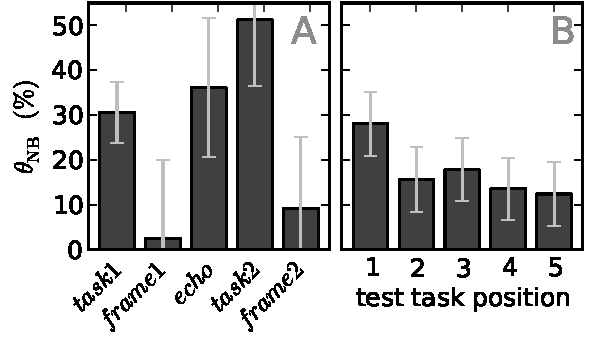
\includegraphics[scale=1]{figs/theta.pdf}
	\caption{
		Bias as measured by a na\"ive Bayes classifier, $\theta_\mathrm{NB}$,
		induced in image-labeling tasks, due to framing and 
		intertask effects. 
		A) Bias in the responses to five test tasks,
		measured between the pairs of treatments indicated on the abscissa.  
		B) Bias between the treatments of \textit{task1}, 
		measured for individual test tasks, and plotted as a function of 
		task position.  Error bars show the 95\% confidence intervals.
	}
	\label{fig:theta}
\end{figure}

To observe the dynamics of intertask effects, we trained a na\"ive Bayes
classifier to distinguish workers in \textit{task1} based on responses to
individual test tasks.  We permuted 
the test tasks to eliminate effects arising from differences in the images 
therein (more details are provided in the supplementary text). The first test 
task shows the greatest bias, after which the effects drop somewhat, but 
substantial bias persists through the fifth test task
(see Fig. \ref{fig:theta}B).  Presumably, this decay profile reflects the
fact that workers are also influenced by their exposure to the test tasks, 
which begins to wash out the effects of initial tasks.

\paragraph{Detailed influences on worker outputs.} 
\begin{figure}
	\centering
	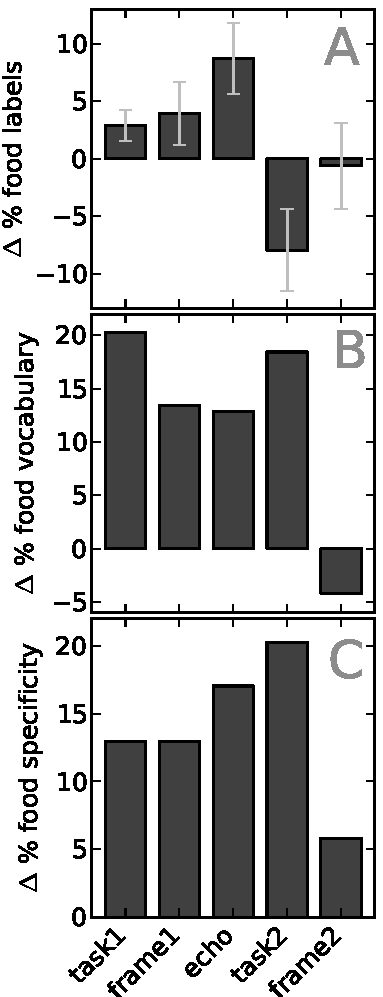
\includegraphics[scale=1]{figs/vocab_specificity.pdf}
	\caption{
		Intertask and framing effects on the vocabulary workers use to refer 
		to food(\#), when labeling images, for various treatment pairs.
		A) Relative change in the number references to food. 
		B) Relative change in the number of \textit{unique} 
		references to food (lexical richness). 
		C) Relative specialization of food references, based on the 
		hypernym-hyponym relations (this calculation is shown in the 
		supplementary text).  For all
		plots, a positive bar height indicates that the \textit{*:food}
		treatment has more of the quantity than its conjugate treatment.
	}
	\label{fig:specificity}
\end{figure}

Using the wordnet corpus, we analyzed exposure effects in finer detail.
Wordnet encodes semantic information in various ways, including in the form 
of synsets (groups of synonymous words), and hypernym-hyponym relations.
Hypernyms are generalizations (``bread'' is a hypernym of ``pumpernickel''),
while hyponyms are specialisations.

First, we used wordnet to identify nouns depicting foods (\# We 
operationalized food-references by taking all hyponyms of the synsets 
\texttt{food.n.01} and \texttt{food.n.02}, with the addition of ethnic foods 
learned by crawling a recipe website, as described in the supplementary text),
to see whether 
workers from the various food-exposed treatments (\textit{*:food}), 
provided more references to food than their conjugate treatments, overall.
The \textit{exp1:*:food} treatments
did produce more food references, but, unexpectedly, 
the number of food references in \textit{task2:food} was
less than that in \textit{task2:cult} (see Fig.~\ref{fig:specificity}A). Also, the effects on the
number of food references was, overall, somewhat smaller than one might 
expect given the extent of bias observed in Fig.~\ref{fig:theta}A.  This means that task and frame exposures
induce other effects which are more subtle than a bulk shift in the number 
of references to the primed concept (food).

Next, we looked at the change in the frequency of occurrence of particular 
words.  Surprisingly, the word ``food'' was the \textit{most suppressed} word
for workers in \textit{*:food} across all treatment pairs (Table S1 shows the
top five most promoted and suppressed words for each treatment pair).
Initially, this seems at odds with the fact that (at least in \textit{exp1})
the \textit{*:food} treatments had more food references than their conjugate
treatments.  But taken together, these facts indicate that workers are opting 
to use more specialized food-references in place of ``food''.  
Indeed, when we look at the total number of unique
words (lexical richness) used to refer to food, we found that 
a significantly richer lexicon was used by all \textit{*:food} treatments,
except in \textit{frame2} (see Fig.~\ref{fig:specificity}B).  This effect 
was especially pronounced in \textit{task1} and 
\textit{task2}.

Finally, we directly calculated the degree of specialization of food 
references using wordnet's hypernym-hyponym relations.  To determine the 
relative specialization between the words of two treatments, we computed 
the proportion of words in the first treatment that were hyponyms of the 
those in the 
second, less those in the first that were hypernyms of those in the second 
(this calculation is formalized in the supplementary text).  Except in the
case of \textit{frame2}, workers in \textit{*:food} treatments used 
substantially more specialized terms in reference to food than workers 
from the conjugate treatments.

\paragraph{Positive and negative priming.}
Taken together, the results of the experiments presented here can be 
explained through a combination of positive and negative priming.
Positive priming (usually simply ``priming'') occurs when a prior stimulus 
predisposes a person to give certain responses in an ensuing task, and
is often observed as an increase in the speed or accuracy of a response, or
the ability to recognize objects in a briefer, quieter, or noisier signal (\#).
Negative priming occurs when, after being repeatedly exposed to a stimulus 
that is perceived to be non-salient, the person begins to ignore that 
stimulus (\#).  

Workers exposed to images containing food will be (positively) primed, 
as memories, concepts, and vocabulary related to food are activated.  
However, we argue that as the worker labels successive images containing food,
the basic 
fact that an image contains food will not appear to be salient, since it 
does not serve to distinguish one image from another.  Thus, the most 
generic references to that fact, such as the label ``food'', 
are suppressed, as by negative priming, while more specialized
references are activated.  Whether workers in \textit{*:food} treatments
produce an excess of food references overall depends in part on the balance 
of these factors.  The reduction in food references from workers in 
\textit{task2:food} relative
to those in \textit{task2:cult} may also be related to the novelty that 
workers in 
\textit{task2:cult} experience when they first encounter food in the test 
tasks.

More generally, we are suggesting that, even though workers are not 
instructed to compare the content of tasks in any way, prior tasks form a 
context relative to which workers judge salience.  Thus, a worker's focus 
in repeated tasks tends to be directed away from generic, shared features, 
toward specific and distinguishing ones.

\paragraph{Recommendations and future work.} 
Based on our observations throughout, we submit the following 
recommendations for the consideration of people designing 
any microtask, citizen science, or crowdsourcing initiative:
\begin{enumerate}
	\item{
		Require active feedback to emphasize important details about the 
		tasks, as we did in \textit{echo1}.  Similarly, use training tasks 
		rather than only examples.
	}
	\item{
		Although ``clean'' examples may be useful to provide clarity,
		use training tasks that contain the same kinds of noise or otherwise
		distracting features as are expected in the real tasks.
		This exposure will negatively prime the worker against non-salient 
		features.
	}
	\item{
		\textit{Validation tasks}, for which the correct output is known,
		are often used as a quality control measure.
		Treat these as \textit{calibration tasks}, and use them to regulate
		the focus of the worker.
		Feedback, for both correct and incorrect responses may further 
		reinforce the desired competency. \label{item:valid}
	}
	\item{
		A special case of item~\ref{item:valid} applies when workers are 
		required to detect rare occurrences.
		For example, in the detection of pre-ictal (pre-seizure) EEG traces, 
		most traces are negative (\#).  In the absence of positive 
		examples, the target concept may degrade or drift.
		Draw calibration tasks from the underrepresented class,
		and provide feedback, to help sustain the worker's target concept.
	}
	\item{
		For more precise classifications, it may help to begin with
		an initial coarse classification.  For example, in detecting 
		inappropriate comments, provide the choices   
		\texttt{okay}, \texttt{inappropriate}, and \texttt{borderline},
		and incentivise inter-worker agreement
		Next, batch the \texttt{borderline}.  Coding this more homogeneous
		borderline set will help workers to calibrate to the finer 
		distinctions necessary for the task.
	}
\end{enumerate}

While these recommendations are informed by the observations we have made 
here, we hope to see them tested directly in future work.

\paragraph{Conclusion.}
We have shown that intertask effects are stronger than framing effects, and
as strong as the effects induced when framing is combined with reiteration.
Intertask and framing effects act on workers' vocabulary in subtle ways.  
Both increase the richness of workers' vocabulary in reference a target
concept, with a more pronounced effect induced by task exposure.
Both exposures also increase the specialization of workers' vocabulary in 
reference to the target concept.  Framing, and other aspects of task design 
have received substantial methodological scrutiny; our results show that 
intertask effects, which were overlooked until now, merit similar 
attention.  Although we found that intertask effects can be a major 
source of bias, they might be used to tune workers' attention and 
specificity relative to
a target concept.  Microtask work, citizen science, and other crowdsourcing
initiatives, as well task requiring expert opinions, often rely on repetitive 
human judgments.  Therefore, such applications all stand to benefit from the 
findings and suggestions presented here.

\bibliography{newbib}
\bibliographystyle{Science}


\section*{Supplementary Material}

\subsection*{S1: Experimental materials}
The tasks for both experiments were presented as a series of slides.  In
both cases, the first slide consisted of a brief set of instructions, followed
by the frame if shown (only some treatments involved a frame), see 
Fig. S\ref{fig:hit_preamble}.  Following the instructions and prime, a set
of initial tasks was shown (except for the treatments in \textit{frame2}
and \textit{echo}) followed by (in all cases) a set of test tasks.  In
\textit{exp1}, two kinds of frame were used, one simple frame, and one where
the worker was required to echo the frame using a combo-box input.  The
instructions, both kinds of frame, and an example task slide, are shown 
in Fig. S1.
\begin{figure}
	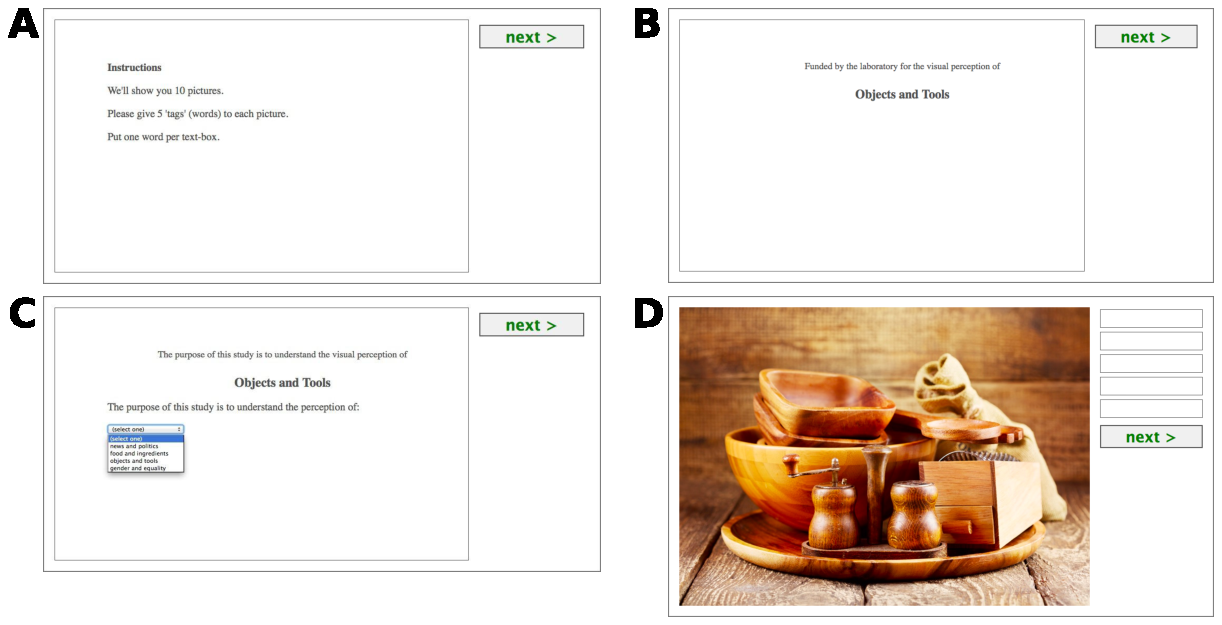
\includegraphics[scale=0.8]{figs/tasks.pdf}
	\label{fig:hit_preamble}
	\caption{Examples of A) instructions; B) a frame, as shown in 
		\textit{frame1:obj}, and similar to those shown in 
		\textit{frame1:food} and \textit{frame2:food}, and 
		\textit{frame2:cult};  
		C) an echoed frame, as used in \textit{echo:obj}, and similar to that
		used in \textit{echo:food}; and D) an 
		example of an image-labeling task.
	}
\end{figure}

All of the initial tasks had the format shown in Fig. S1D.  The images used
in the initial tasks for \textit{task1:food} and \textit{task1:obj} are
shown in Fig. S2 and S3, and the images used in the test tasks for 
\textit{exp1} are shown in Fig. S4.  The images used in the initial tasks
for \textit{task2:food} and \textit{task2:cult} are shown in Fig. S5 and
Fig. S6 respectively, and the images used in the test tasks for \textit{exp2} 
are shown in Fig. S7.

\begin{figure}
	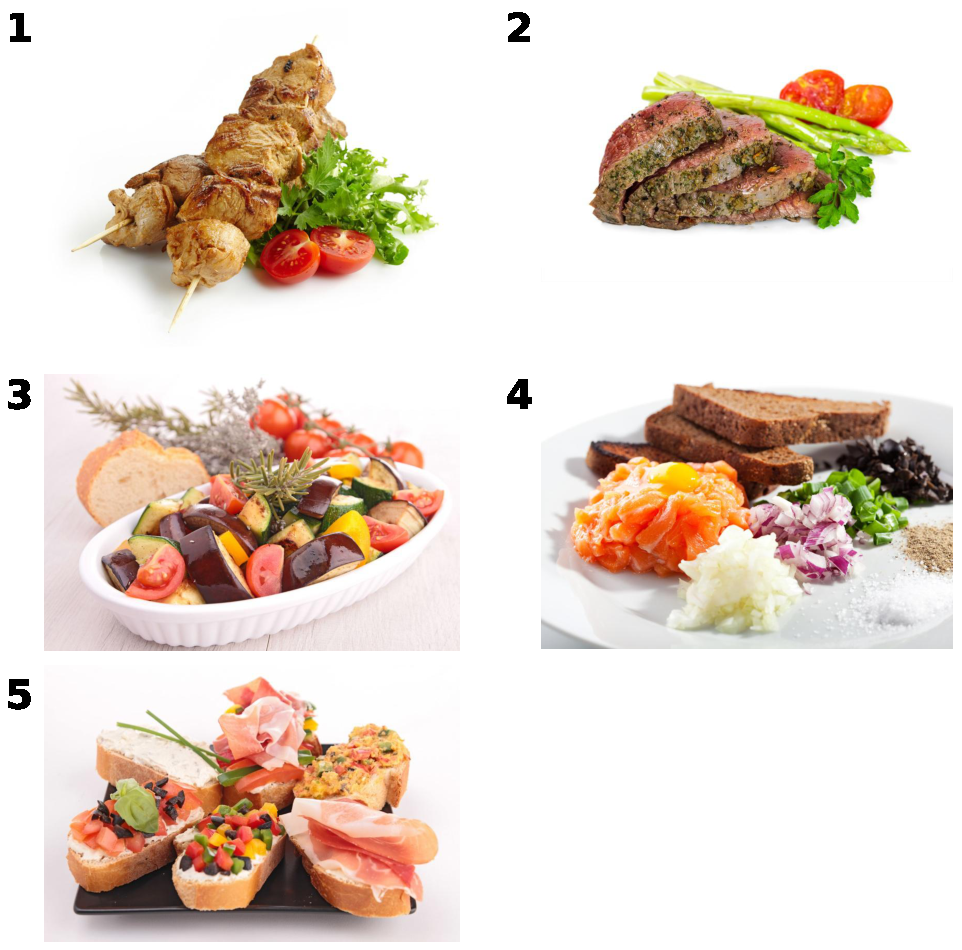
\includegraphics{figs/task1-food.pdf}
	\label{fig:task1:food}
	\caption{
		Figure S2: Images used in the initial tasks for 
		\textit{task1:food}.  The numbers show the order in which the 
		images were presented to workers.
	}
\end{figure}

\begin{figure}
	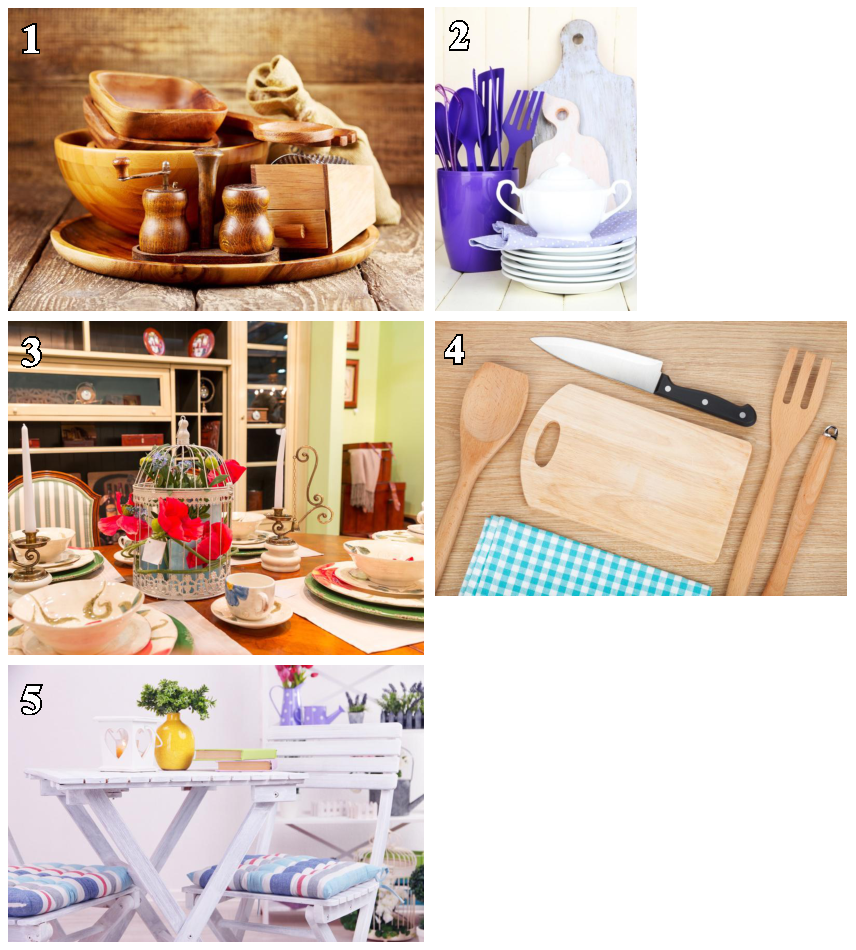
\includegraphics{figs/task1-obj.pdf}
	\label{fig:task1:obj}
	\caption{
		Figure S3: Images used in the initial tasks for 
		\textit{task1:obj}.  The numbers show the order in which the 
		images were presented to workers.
	}
\end{figure}

\begin{figure}
	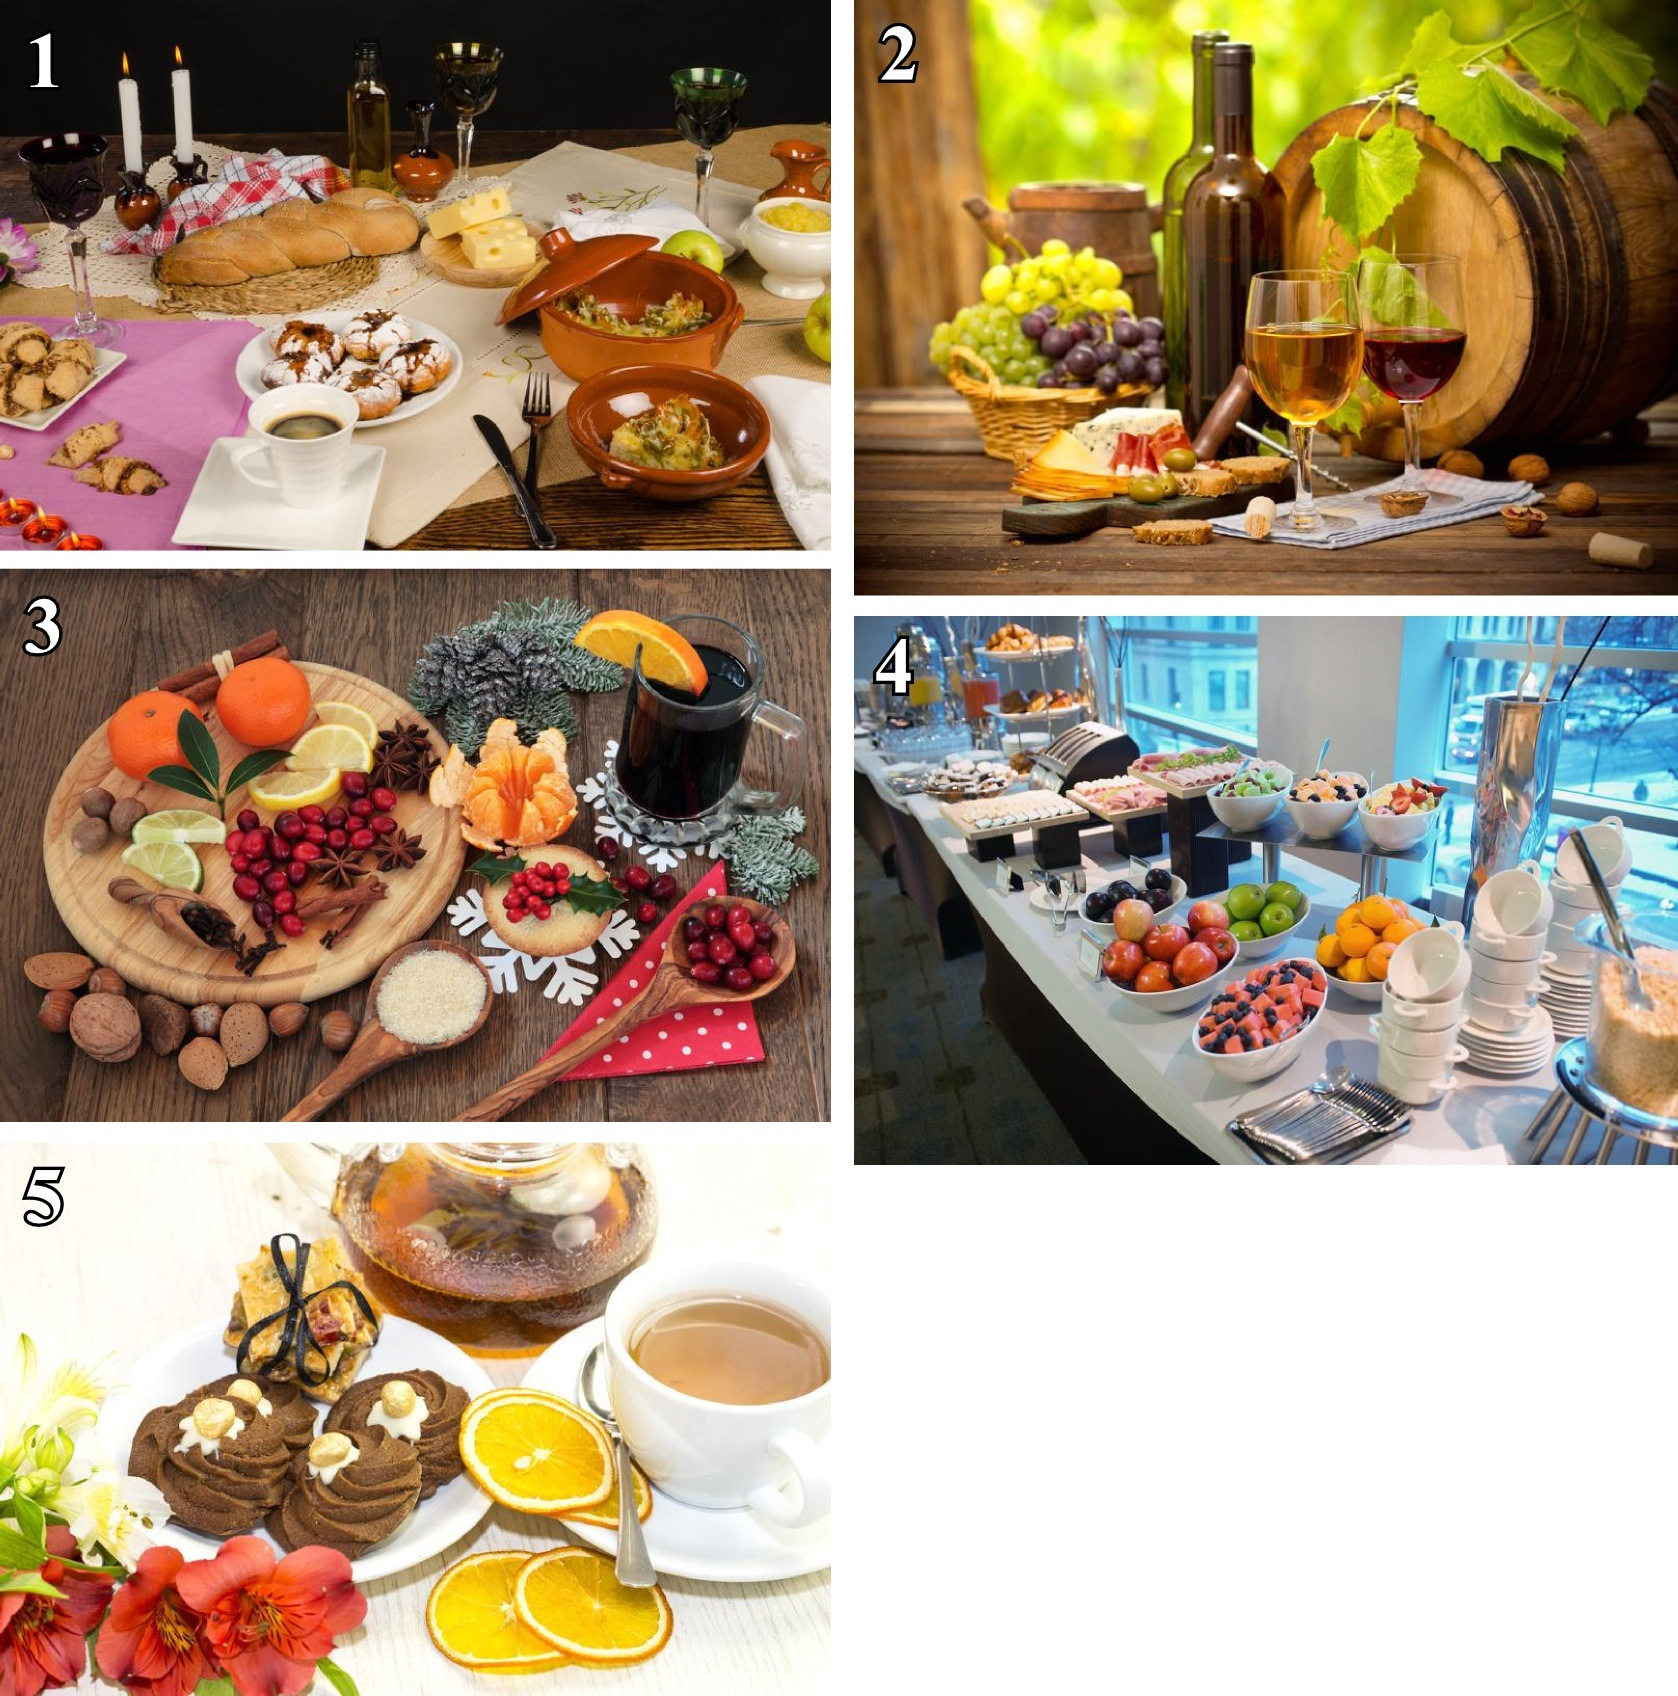
\includegraphics{figs/task1-test.pdf}
	\label{fig:task1:test}
	\caption{
		Figure S2: Images used in the test tasks for 
		\textit{exp1}.  The numbers show the order in which the 
		images were presented to workers.
	}
\end{figure}

\begin{figure}
	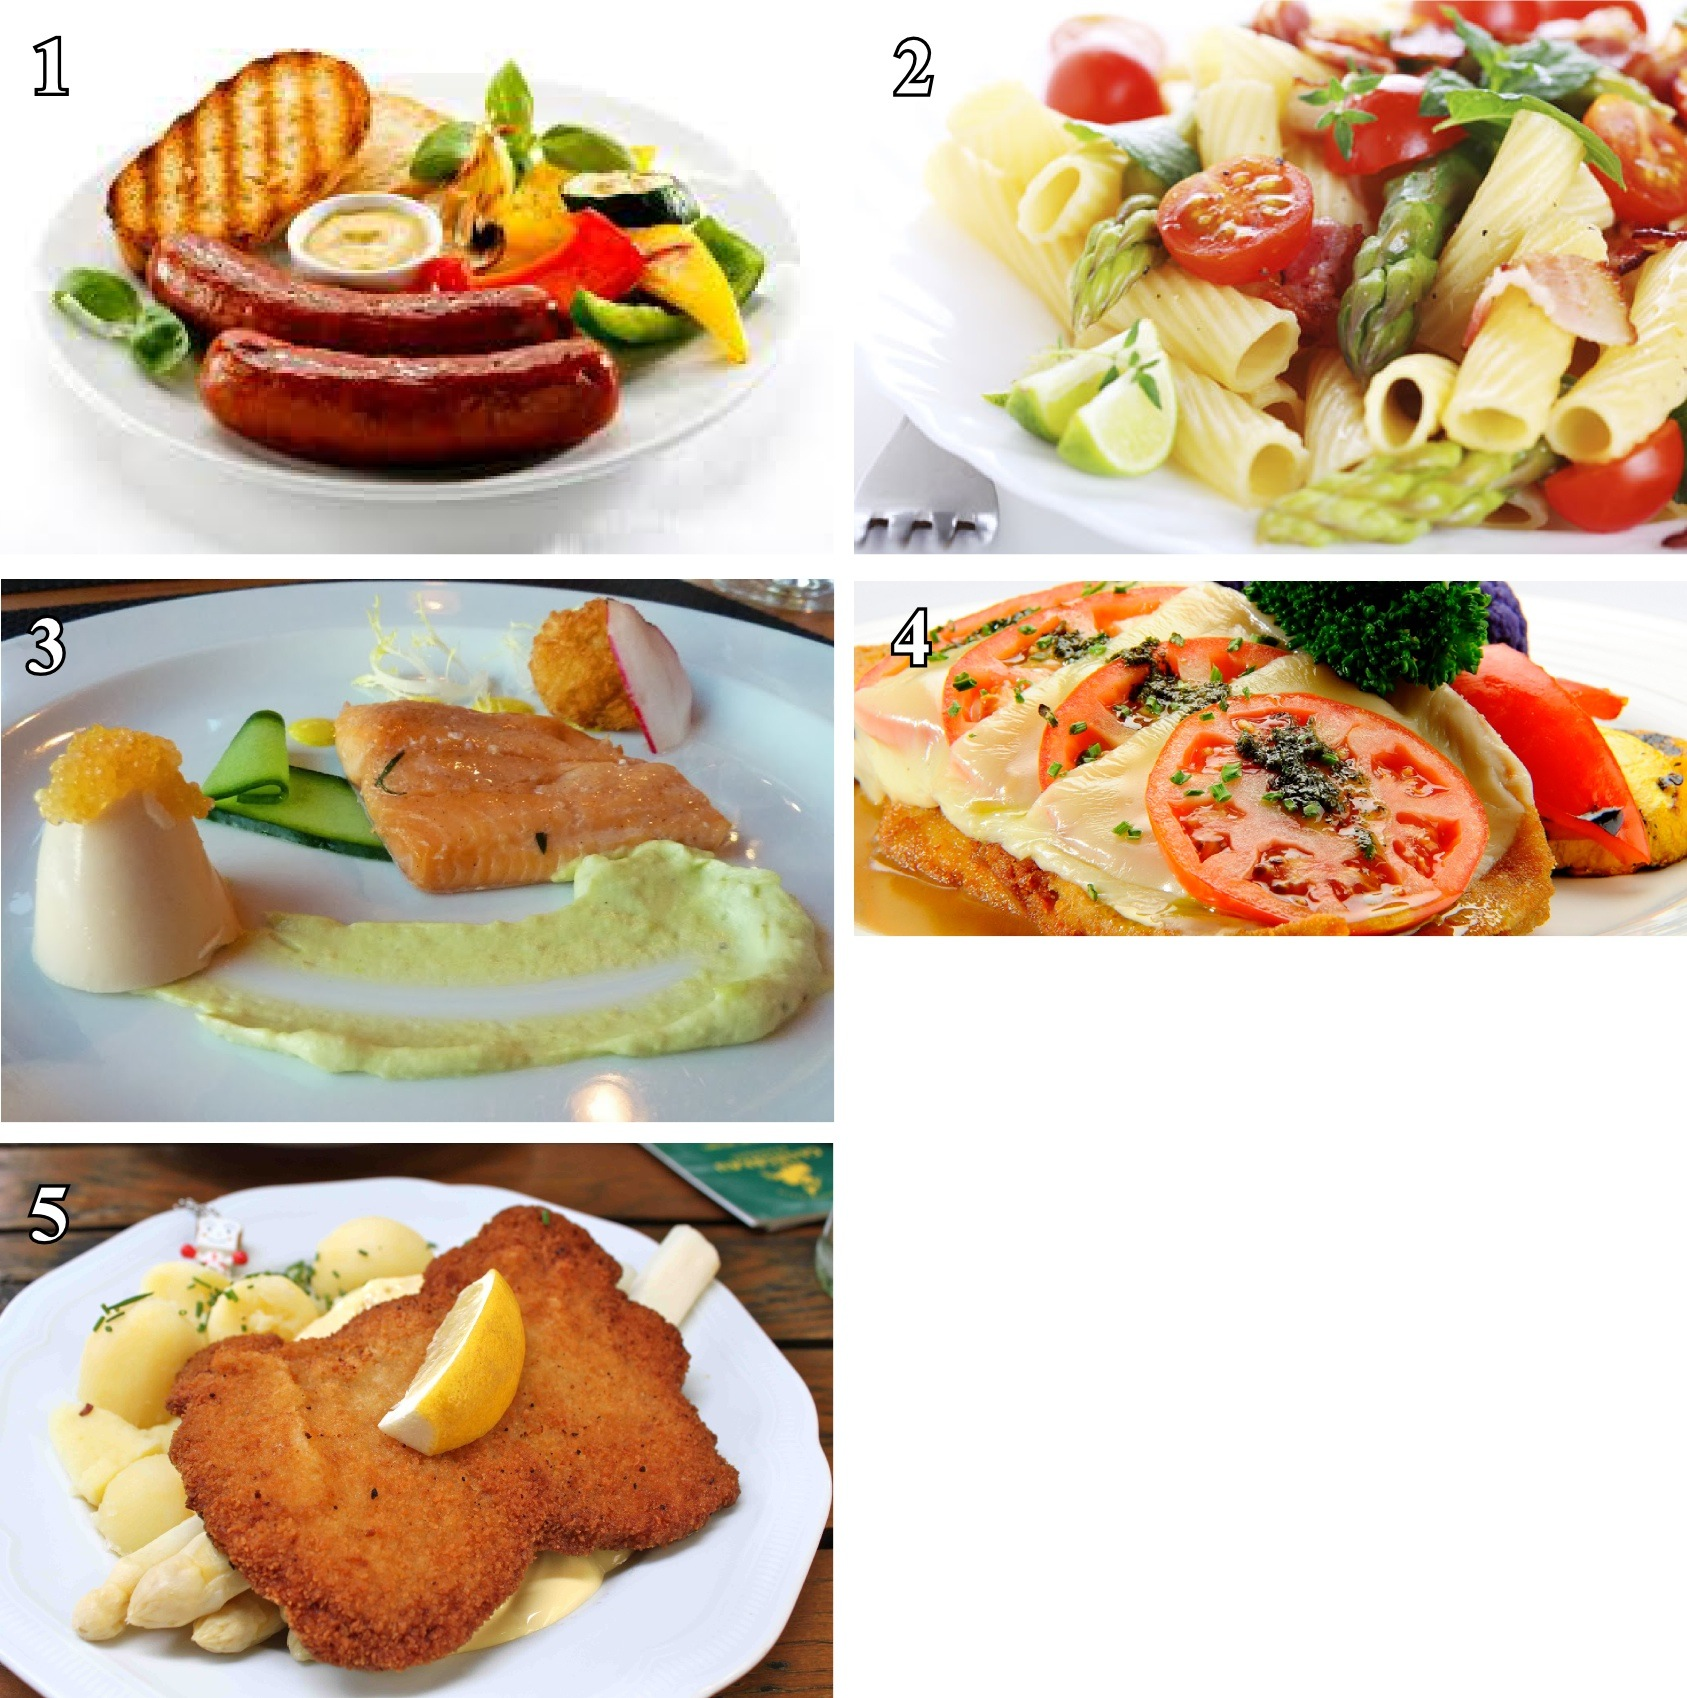
\includegraphics{figs/task2-food.pdf}
	\label{fig:task2:food}
	\caption{
		Figure S2: Images used in the initial tasks for 
		\textit{task2:food}.  The numbers show the order in which the 
		images were presented to workers.
	}
\end{figure}

\begin{figure}
	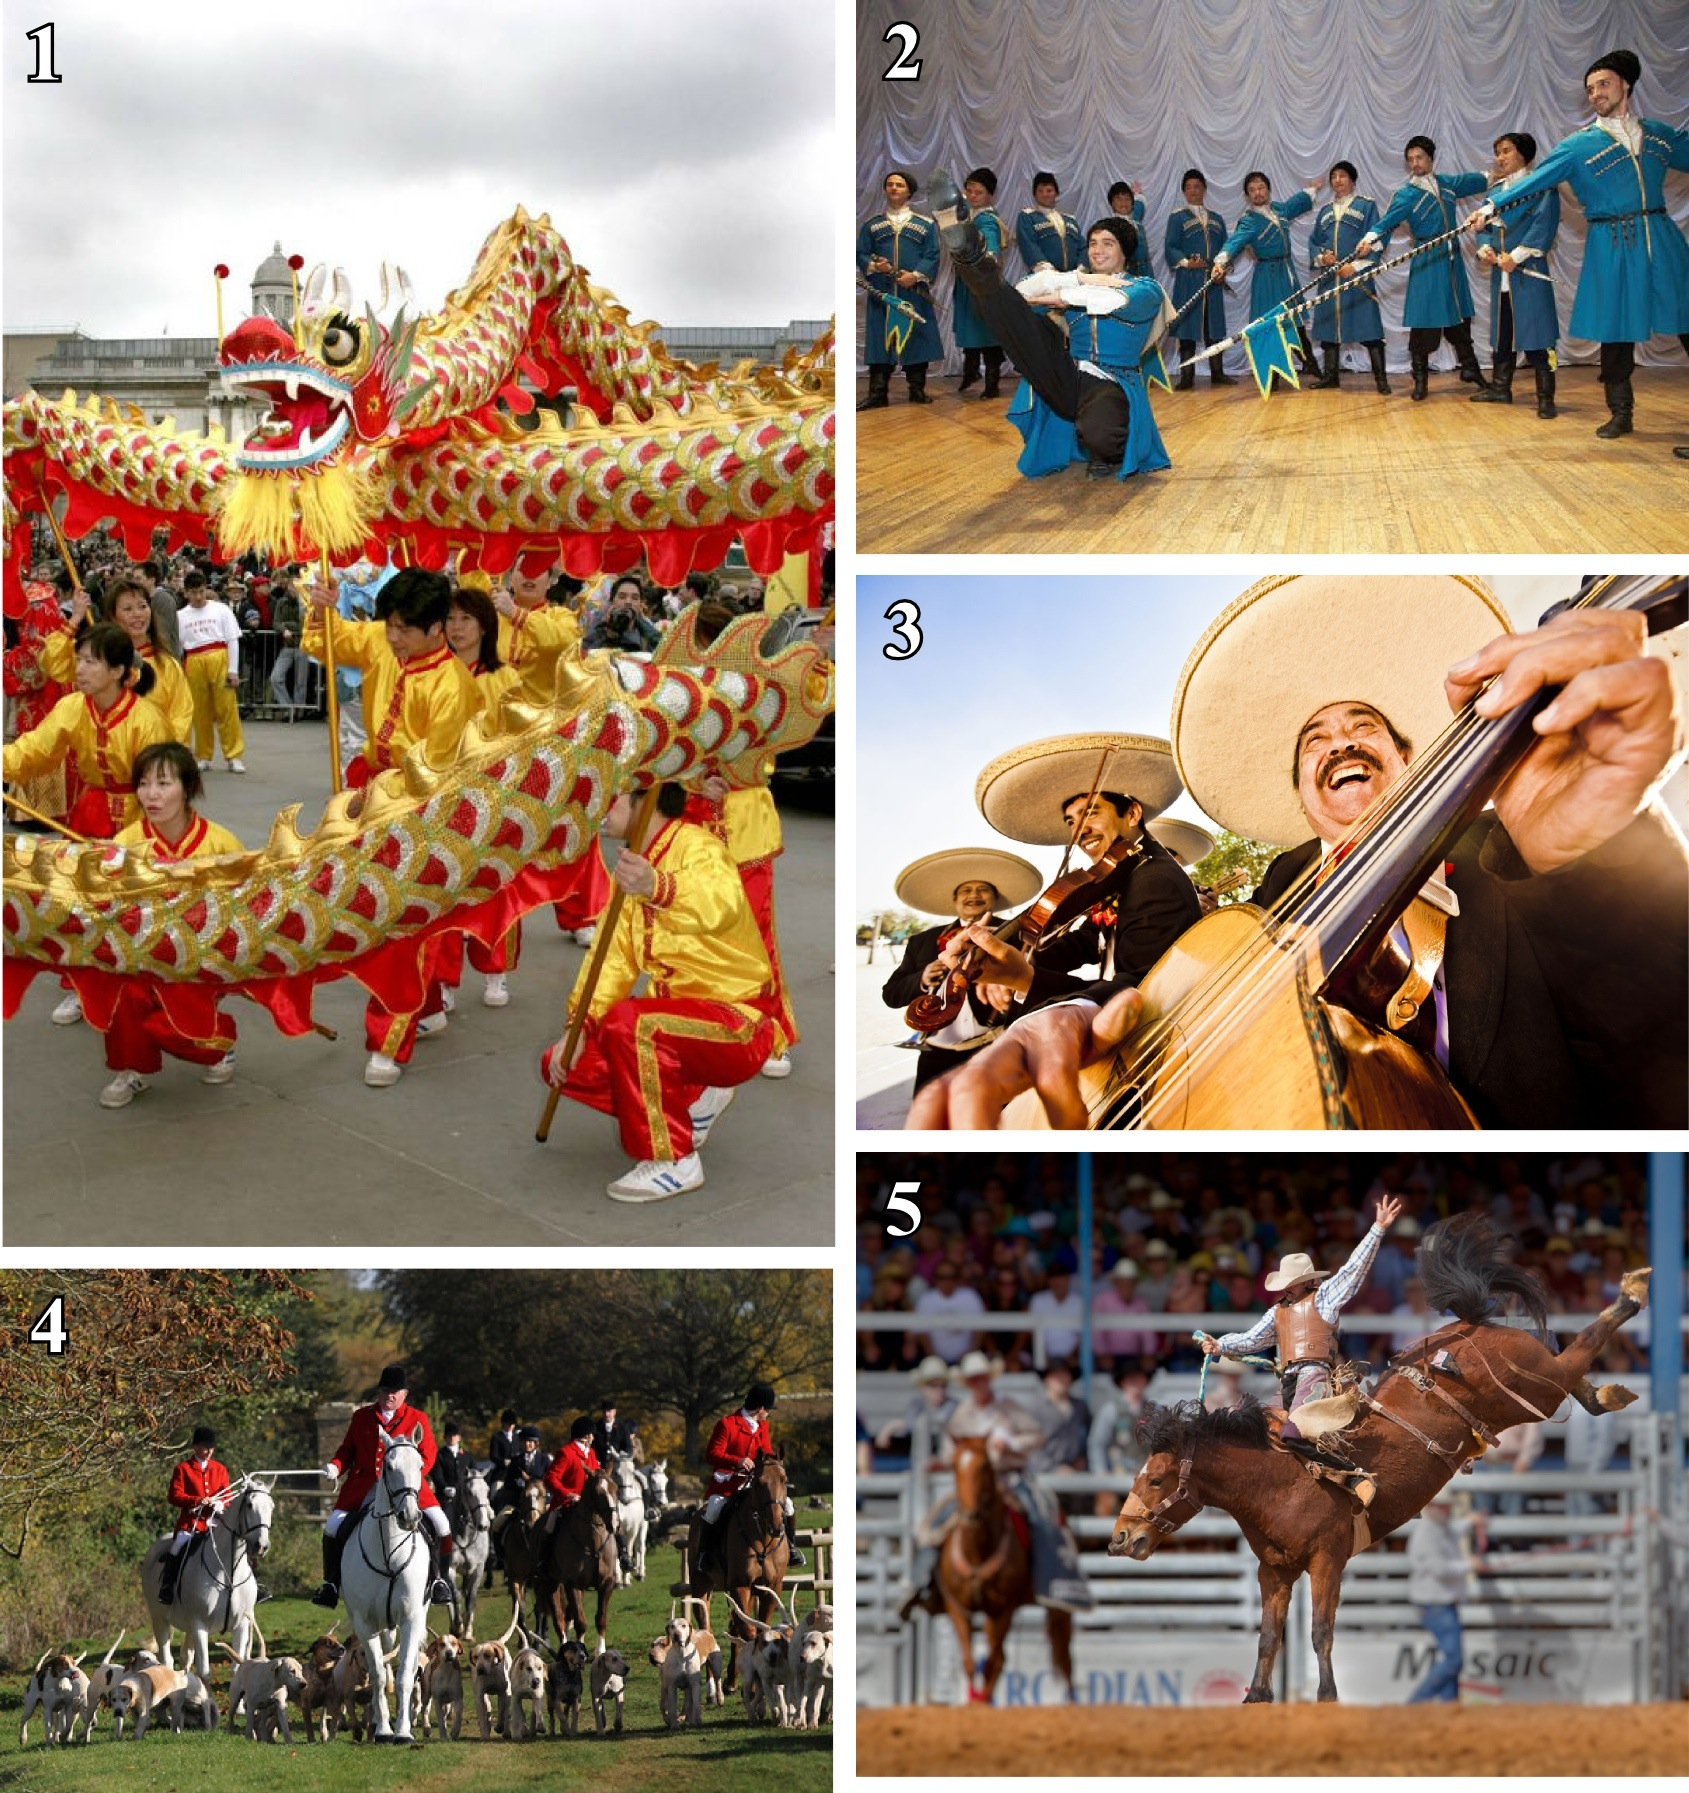
\includegraphics{figs/task2-cult.pdf}
	\label{fig:task2:cult}
	\caption{
		Figure S2: Images used in the initial tasks for 
		\textit{task2:cult}.  The numbers show the order in which the 
		images were presented to workers.
	}
\end{figure}

\begin{figure}
	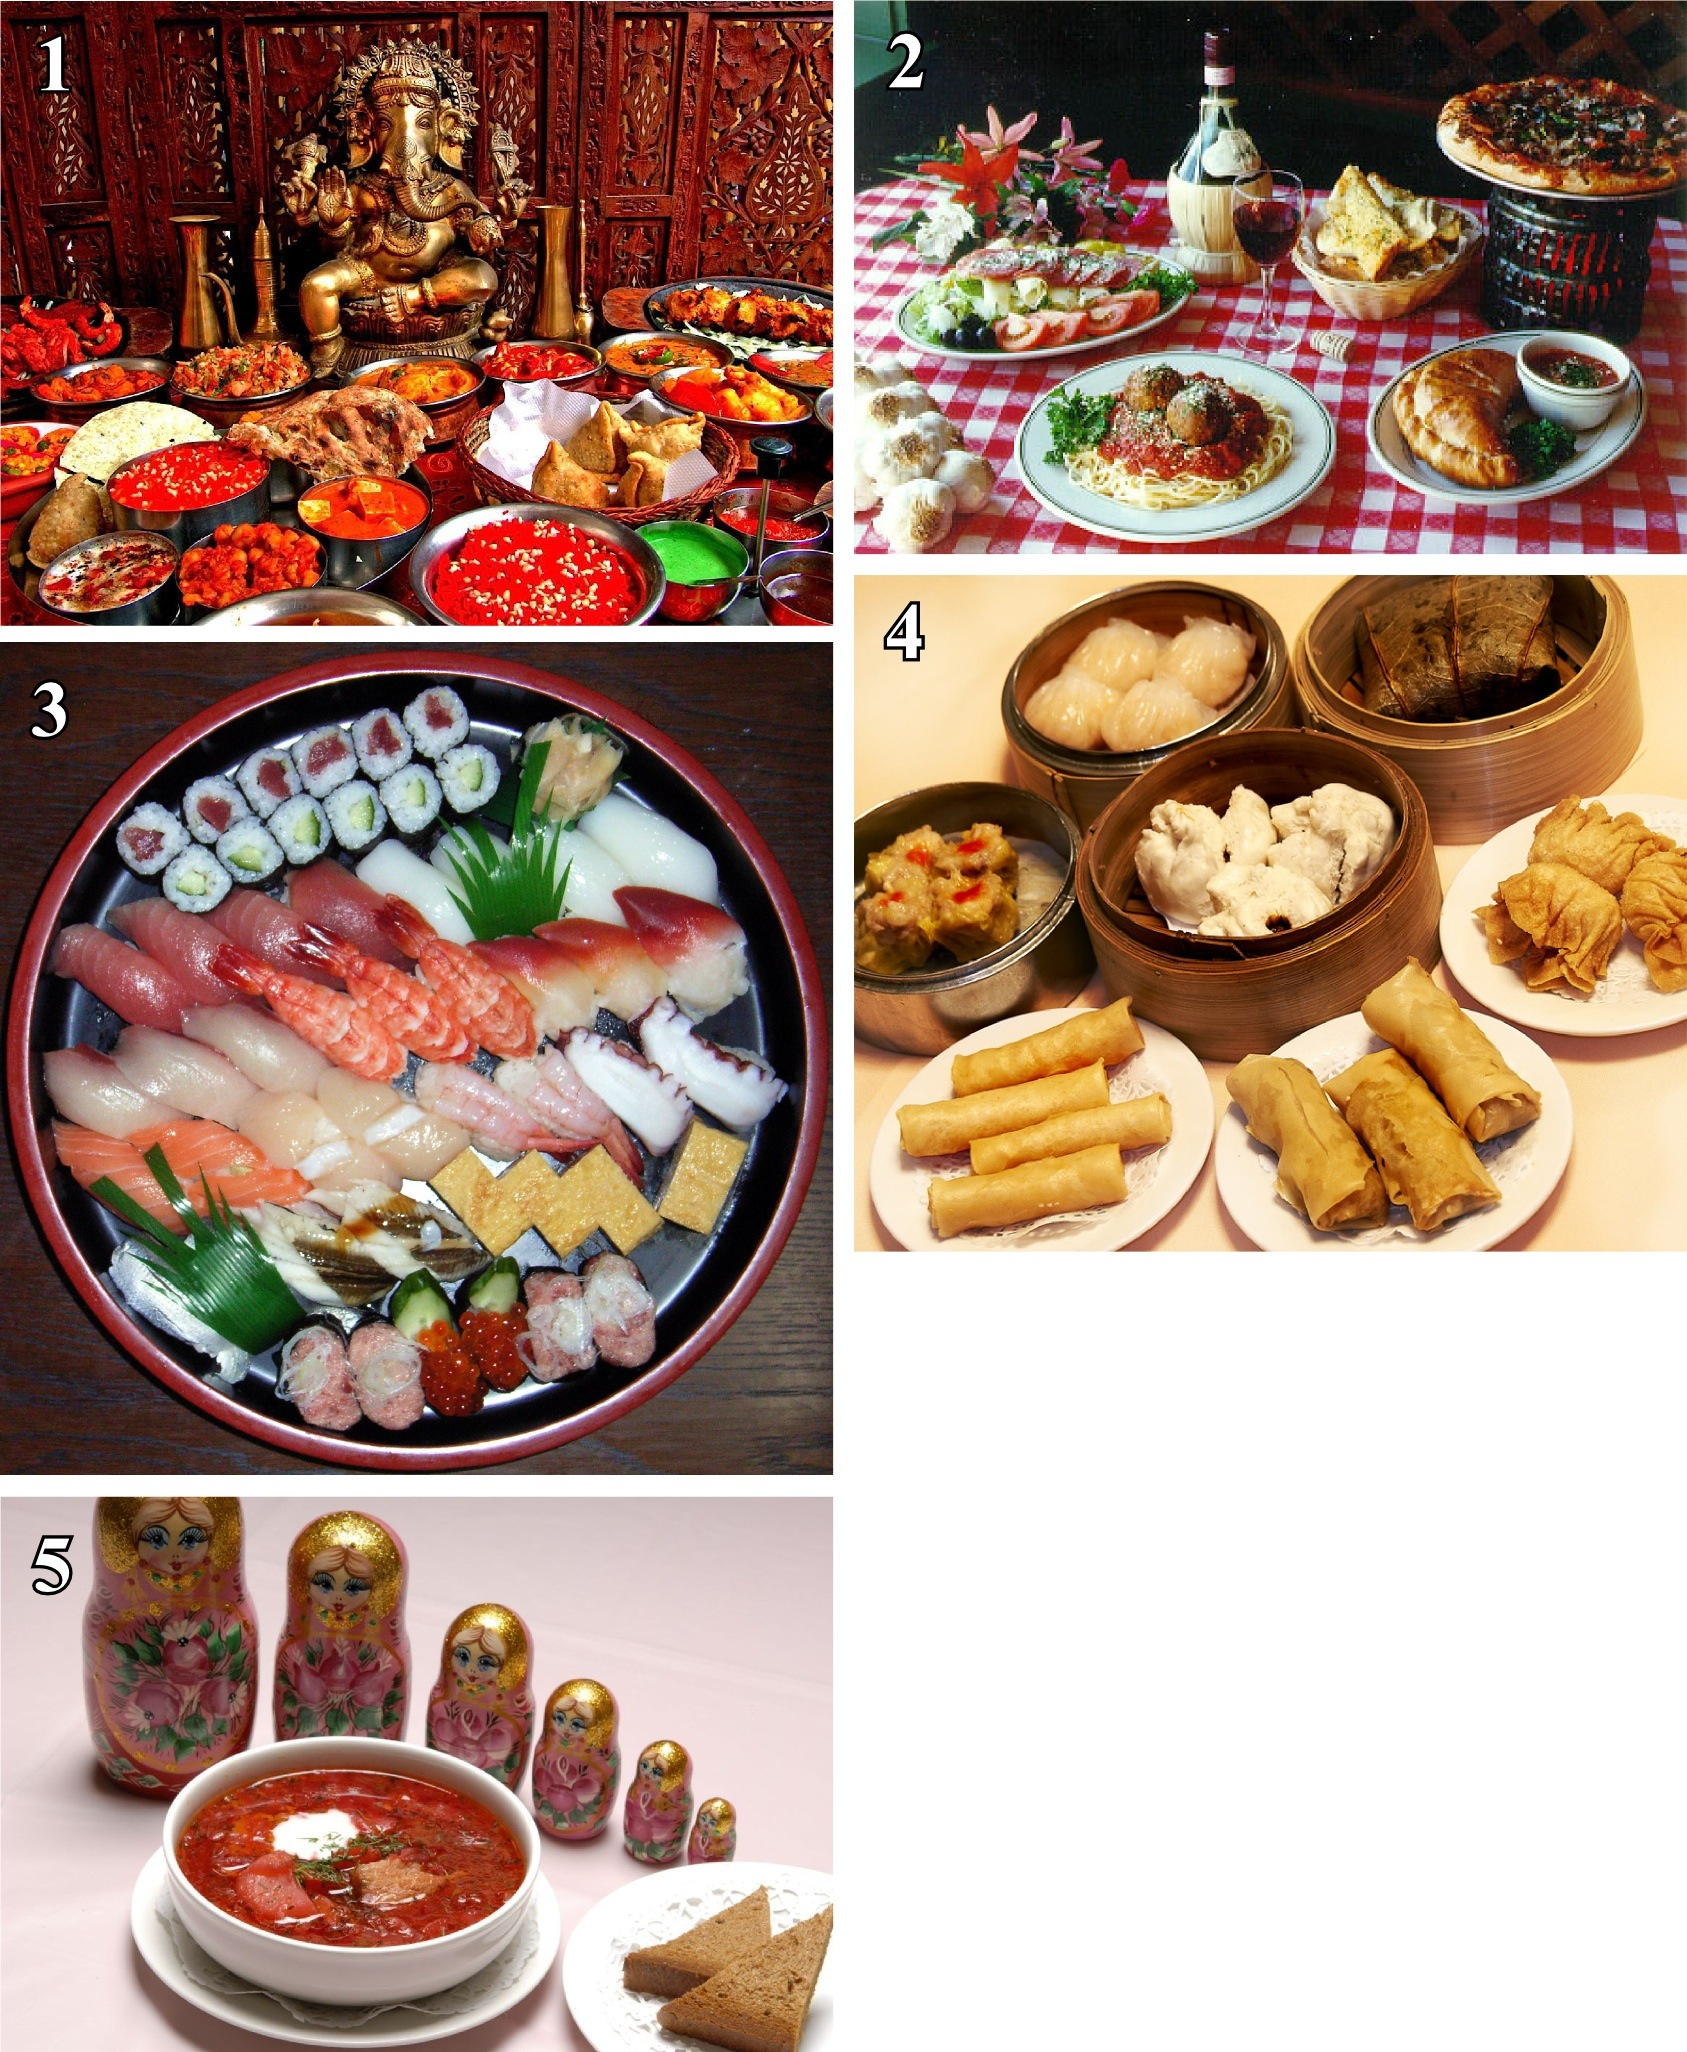
\includegraphics{figs/task2-test.pdf}
	\label{fig:task2:test}
	\caption{
		Figure S2: Images used in the test tasks for 
		\textit{exp2}.  The numbers show the order in which the 
		images were presented to workers.
	}
\end{figure}

\subsection*{S2: Access to raw data and code}
The raw data and source code needed to reproduce the analyses 
shown here and in the main text can be downloaded from 
http://networkdynamics.org/publications/public/priming2014.09.

\subsection*{S3: Additional results not shown in the main text}
		the top 5 most suppressed and most activated terms between treatment
		pairs.

\begin{table}
	\centering
	\setlength{\tabcolsep}{10pt}
	\begin{tabular}{ c c c c c }
	
		\setlength{\tabcolsep}{4pt}
		\begin{tabular}{ r | c }
		\toprule
		\multicolumn{2}{c}{\textit{task1}} \\
		\toprule
		coffee & 38 \\
		meal & 34 \\
		cheese & 34 \\
		apple & 32 \\
		dessert & 21 \\
		cup & -30 \\
		glass & -45 \\
		table & -70 \\
		candle & -74 \\
		food & -80 \\
		\bottomrule
		\end{tabular}

&

		\setlength{\tabcolsep}{4pt}
		\begin{tabular}{ r | c }
		\toprule
		\multicolumn{2}{c}{\textit{frame1}} \\
		\toprule
		bread & 18 \\
		wine & 18 \\
		cheese & 16 \\
		apple & 14 \\
		oil & 12 \\
		table & -9 \\
		meal & -10 \\
		candle & -12 \\
		dinner & -13 \\
		food & -32 \\
		\bottomrule
		\end{tabular}

&

		\setlength{\tabcolsep}{4pt}
		\begin{tabular}{ r | c }
		\toprule
		\multicolumn{2}{c}{\textit{echo}} \\
		\toprule
		apple & 24 \\
		cheese & 23 \\
		wine & 15 \\
		coffee & 14 \\
		oil & 7 \\
		knife & -24 \\
		dinner & -26 \\
		fork & -27 \\
		candle & -35 \\
		food & -55 \\
		\bottomrule
		\end{tabular}

&

		\setlength{\tabcolsep}{4pt}
		\begin{tabular}{ r | c }
		\toprule
		\multicolumn{2}{c}{\textit{task2}} \\
		\toprule
		spicy & 26 \\
		sauce & 17 \\
		indian & 15 \\
		buffet & 14 \\
		exotic & 12 \\
		festival & -11 \\
		offering & -12 \\
		statue & -15 \\
		india & -20 \\
		food & -56 \\
		\bottomrule
		\end{tabular}

&

		\setlength{\tabcolsep}{4pt}
		\begin{tabular}{ r | c }
		\toprule
		\multicolumn{2}{c}{\textit{frame2}} \\
		\toprule
		indian & 11 \\
		banquet & 8 \\
		spicy & 7 \\
		asian & 6 \\
		variety & 6 \\
		delicious & -6 \\
		meat & -7 \\
		festival & -7 \\
		spice & -7 \\
		food & -9 \\
		\bottomrule
		\end{tabular}

	\end{tabular}
	\caption{blah}
\end{table}

\subsection*{S4: Data preprocessing}
	\paragraph{Splitting, Lemmatization, removal of stop-words, and 
		addition of position tags.} 

	Before performing any analysis on the labels that workers provided, we
	performed a series of preprocessing steps.  
	\td{does this reflect the actual order in which the steps were done?}
	First, words wore lematized 
	using the
	\td{whatzit} lemmatizer.  This lemmatizer is very mild, tending only to 
	change plural words to their singular form.  Common
	words such as ``the'', ``to'', or ``with'', were found using the
	the \td{whatzit} stop-word list and removed.  Then, misspelled words were
	automatically corrected using a spelling correction algorithm described 
	below.  Finally, labels that contained
	multiple words (separated by spaces or punctuation) were split, with
	punctuation removed, and the separated words were treated as distinct 
	features in subsequent analysis.

	For the purpose of training and testing a na\"ive Bayes classifier, we 
	performed an additional preprocessing step.  We tagged words with the
	position in which they had been entered (i.e. which of the five text 
	inputs in the task interface) as well as the test tasks in which the word 
	had been provided.
	So, if the word ``wine'' was entered into the second text-input for 
	the third test-task, after preprocessing, the feature ``3\_2\_wine'' would
	appear.  Prepending the task number onto words was simply a means to 
	retain correct attribution, which itself was essential since providing a
	word during one task is not equivalent to providing the same word during 
	another task.  
	
	\paragraph{Spelling correction.}  
	Spelling correction was performed using an algorithm that first detected
	if a word was likely to be misspelled, then generated a set of candidate 
	corrections, and chose the best candidate based on a scoring mechanism.
	
	A word was considered misspelled if it was not contained in the 
	\textit{legal set}, which was formed by the union of
	the wordnet corpus, the stop-word list, and a set of words seen while 
	crawling the world food section of the allrecipes.com website.  We
	describe the crawling of the allrecipes.com website in a section below.

	To correct misspellings, we first produced all possible modified forms 
	that could be obtained applying one or two edits.  An edit consisted of 
	adding or removing a letter, changing one letter into another, or 
	swapping the positions of two adjacent letters.  For the purpose of these 
	edits, spaces were treated as any other letter.

	The candidates produced by these edits which were in the legal set were
	then ranked based on a scoring mechanism, and the highest scoring word
	was chosen as the correction.  A candidate $w$'s score, $s_w$, was 
	calculated according to the following formula:
	\begin{equation}
		s_w = (f_w + 1) * p_1 * p_2,
	\end{equation}
	where $f_w$ is the frequency with which the word occurred (correctly 
	spelled)
	within the given task, $p_1$ was a penalty for the first edit, and
	$p_2$ was a penalty for the second edit.  If the word was made using only
	one edit, then $p_2 = 1$.  Any edit that did not involve adding a space
	(i.e. separating a word) incurred a penalty of 0.5, while the addition of
	a space incurred a penalty of 0.1.  Word-separation edits were more 
	strongly penalized because it is often possible to split a series of 
	letters into many short two- or three-letter words, which otherwise leads 
	to many erroneous corrections.  We found that setting the penalty for
	word splitting at 0.1 worked well by testing on words taken from
	initial tasks.

	After all of our analyses had been performed, we checked the accuracy of 
	the spelling correction algorithm using three human coders.  The coders
	were shown a set of 
	500 words that were randomly sampled from the labels attributed during 
	test tasks (50 for each test task).  Before sampling, the labels from all
	experimental treatments, for the given test task, were pooled together.
	The coders did not know which treatment any given word came from.  
	In addition to the words, coders were shown the spelling correction 
	produced by the algorithm, as well as the image from the test task.
	The coders were asked to identify any misspelled words which had not 
	been corrected, as well as any corrections that appeared to be erroneous,
	by indicating their own correction.

	Based on this exercise, we found that, according to the human coders,
	17\% of the words were misspelled, but that after applying the 
	automated spelling correction, only 3.2\% of words were misspelled.

	\paragraph{Crawling the world food section of allrecipes.com.}
	The website allrecipes.com was accessed on 3-4 November 2014 using 
	automated scripts.  A total of 2642 recipe listings and 15621 recipe
	instruction pages were crawled.  Recipe listings were pages that provided 
	lists of recipes, and contained a title and short description for each.  
	The recipe instruction pages had lists of ingredients and preparation 
	instructions.  All of the words found in recipe titles, short
	descriptions, ingredients lists, and preparation instructions were
	collected, and saved as an auxiliary set to augment the \textit{legal set}
	used in spelling correction.
	


\subsection*{S5: Identification of food-related terms}
The wordnet corpus is composed of synsets, which are particular senses 
(meanings) and a set of word forms bearing that meaning. A given word form, 
such as ``ring'' has multiple senses (``to ring a bell'', ``a wedding ring''), 
and so can be part of many synsets.  Since the wordnet corpus was designed
to carry semantic information, the synset is the basic organizing element
of wordnet.

We chose the synsets \textit{food.n.01} and \textit{food.n.02} to act as roots
in defining which words should be considered food-related.  Any word form
belonging to a synset which was a hyponym of one of the two root synsets
identified above was considered to be a reference to food.  Here, as in the
main text, when we say hyponym, we mean either a direct hyponym, or a hyponym
of a hyponym, and so on.

This is a stringent notion of a word being a food reference.  It roughly
corresponds to whether or not a given thing is reasonably considered 
consumable.  So, ``orange'' is food, but ``salty'' is not.  Although ``salty''
would usually refer to something edible, it is not itself an edible thing.
On the other hand, ``salt'' would be considered a reference to food under 
this operationalization.

The subset of the wordnet corpus induced by the hyponyms of \textit{food.n.01}
and \textit{food.n.02} provide an extensive set of \td{X} words.  Manual
testing appeared to show that the coverage was very extensive, except in 
some cases references to ethnic foods were missing.  Since, especially in
\textit{exp2} we had images containing many ethnic foods, we decided to 
augment the wordnet corpus with words learned by crawling the world food
section of the allrecipes.com website.  

After collecting a set of words using an automated script 
(\td{described above}), we collected the set of words that had been used by
workers and which had been seen during crawling of the allrecipes.com website,
but which were not included in wordnet.  We grafted these extra words into
the wordnet hyponym-hypernym graph manually, which ensured that any references
to ethnic words learned from crawling would be properly classified as 
food references.

\paragraph{Validation of the detection of food references.}
To determine whether our extended version of wordnet provided a good approach
to detecting food-related words, we sampled 500 words from the set of labels
produced by workers and had three human coders manually decide if they were 
food-related or not.  The method for randomly sampling the 500 words was 
described in above in \td{section number}.

The coders were instructed to consider whether a word was a noun signifying
an edible item.  The guiding principle was, for the coder to ask herself,
``can I eat this X'', where X is the word she is coding.  The coders were
shown the used in the task from which the word came, to help resolve ambiguity
in the sense of the word that had been given.  Coders were also shown the 
spelling correction (if any) that the spell-correction algorithm had made,
to help interpret misspelled words \td{we describe the spelling correction 
algorithm in section X}.

We evaluated the food detection algorithm in two ways.  First, we measured
the inter-rater reliability between the three human coders and the algorithm
(treating the algorithm just like any other coder).  Second, adopting the 
majority code given by the human coders, we determined the accuracy of the
food-detection algorithm.  Data summarizing this validation process are given
in table S1.

\begin{table}
\centering
\setlength{\tabcolsep}{12pt}
\begin{tabular}{ r | c }
\toprule    
\# terms coded & 500 \\
\# food references & 130 \\
\# correct machine codes & 440 \\
inter-rater reliability & 82.4\% \\
human-machine code agreement & 88\% \\
%machine recall & 80 \% \\
%machine precision & 75.4 \% \\
%machine code F1 & 0.78 \\
\bottomrule
\end{tabular}
\caption{\footnotesize{
	\td{remove the automatic numbering}. Table S1. Results for the validation 
	of the automatic detection of food references, by comparison to
	human-generated coding on randomly sampled words.  In calculating the 
	human-machine code agreement, the majority human code was used.
	Inter-rater reliability was calculated as Krippendorff's alpha.
}}
\end{table}

The results show that good inter-rater reliability was achieved during the
validation (82.4\%).  Looking at the agreement between the 
machine codes and the majority human-generated codes, we find they agree
88\% of the time.  This means that the concept used to instruct human coders
provides a good approximation to what the wordnet-based machine codes actually
represent. In other words, the machine codes correspond closely to indicating
which words correspond to nouns that refer to edible things, and which ones
don't, which provides a clear and simple interpretation for the machine
coding of food and non-food words.

\subsection*{S6: Calculation of relative specificity}
In the main text we present results for the relative specificity of labels
produced by two experimental treatments.  In performing this calculation,
we used the wordnet corpus, which has a set of hypernym-hyponym relationships
as described in the main text.  The first step in performing this calculation
was therefore to map the words occurring from (the labels of) a given 
experimental treatment onto the wordnet synsets.  In general, a given word
form can have multiple meanings, and therefore maps onto multiple wordnet 
synsets.

The result of mapping the words from two treatments onto the wordnet 
hypernym-hyponym graph two sets of counts, one set per treatment, 
indicating the number of times a word from a given synset occurred among the
labels of the treatment.  Then, for every synset in one treatment, we looked
at the number of synsets in the other treatment that were more generic
(reachable by following hypernym relations) less the number of words that
were more specific (reachable by following hyponym relations).  This quantity
tallied for all words in the original synset gives a (non-normalized) measure
of the degree to which words from the first treatment are more specific
than words from the second treatment, overall.  We then normalized this 
quantity by the total number of possible comparisons between the words of
one treatment to those of the other, where two words are considered comparable
only if one word is the hypernym or hyponym of the other.  Hence, ``statue'' 
and ``bread'' are not comparable, but ``pumpernickel'' and ``bread'' are.

This calculation can be summarized by the following equation:
\begin{equation}
	S(P,Q) = \frac{
		\sum_{w\in P}\sum_{v\in Q} \left(
			\mathbf{1}_{[w>v]} - \mathbf{1}_{[v>w]} \right)
	}{
		\sum_{w\in P}\sum_{v\in Q} \left(
			\mathbf{1}_{[w>v]} + \mathbf{1}_{[v>w]} \right)
	},
\end{equation}
where $P$ and $Q$ are sets of synsets, and $\mathbf{1}_{[w>v]}$ evaluates
to 1 if synset $w$ is more specific than (i.e. is a hyponym of) synset $v$.
This measure counts the excess of cases where synsets from $P$ are more
specific then synsets from $Q$, as a fraction of all comparable synset pairs. 

In computing this quantity between two treatments, we first computed it 
using the labels attributed to a particular test task, and then
averaged the result obtained in this way for each of the five test tasks.

\subsection*{S7: Analysis of variance}
	\paragraph{Variance in the average fraction food-related labels}
	In the main text, Fig.~\ref{fig:specificity}A shows the difference in 
	the fraction of food related labels used by workers in from different 
	treatments.  The error bars show the 95\% confidence intervals around 
	the estimated difference of means.  It was computed from the
	observed sample standard deviation in the fraction of food labels given
	by individual workers.

	\paragraph{Variance in food vocabulary size.}
	\td{Not sure how to calculate this yet.}

	\paragraph{Variance in food specificity.}
	\td{Need to calculate this using bootstrapping.}


\subsection*{S8: Measuring computational hysteresis}
	\paragraph{Using cross-validation accuracy to lower-bound L1-distance.}
	In order for Eq.~\ref{l1} to be applicable, it is necessary to obtain
	an unbiased estimate of a classifier's performance.  One well-known
	pitfall in measuring this error is to underestimate it due to 
	over-fitting of the data used.  As an example, if one were to try 
	a large number of classifiers, eventually one would find one that
	classifies the data perfectly, even though it might non generalize to
	new data.

	It is customary to use part of a data set to optimize hyperparameters of
	a model, and then test the model on as-yet unseen data.  In our case,
	don't have enough samples in each treatment to do this.  Instead, for 
	this reason, we make principled decisions for all of the options used
	in our classifier, and then test it's accuracy using cross validation,
	with no optimization performed on the data.  It was crucial for 
	the statistical validity of our approach that we test our classifier on 
	each datum only once, and report these results without any optimizations
	of the classifier.

	In performing the classification we had various options, and since we
	could not optimize these choices, we made principled decisions based on
	prior knowledge from text classification applications.  We describe the
	options we faced and the choices we made below.

	\textit{whether to correct misspelled words.}  Because we used free-text
	entry for the labels, there was bound to be many spelling mistakes.
	This would tend to reduce the accuracy of a classifier, because the 
	entries ``bread'' and ``braed'' would be regarded as completely different
	features, even though they clearly correspond to the same 
	\textit{intended word}.  While no algorithm can determine a worker's 
	intentions, it is possible to check words against a corpus, and, in the
	case of a misspelled word, look for plausible corrections based on 
	edit distance.

	\textit{Lemmatization.}  In some cases it is helpful to simplify words 
	before providing them to the classifier.  For example, the words 
	``berries'' and ``berry'' only differ in number, but would normally be
	treated as completely different features.  Lemmatization ensures that
	nouns are in their singular form, which helps to eliminate variations in
	labels that increase sparsity without conveying discriminative 
	information.

	\textit{Removal of stop-words.}  Certain very common words such as `the',
	``to'', and ``it'' are extremely common but don't help discriminate a 
	worker's exposure.  Removing these words is a common practice because
	they otherwise introduce noise into the classifier learning process.

	\textit{Whether to split multiple words.}  Although workers were 
	instructed to put one word per text input, many put multiple words.
	Theoretically the original multi-word entry might bear additional 
	information that could be useful in discerning a worker's exposure. 
	In practice, it would be necessary for that word combination to recur,
	which is unlikely.  Therefore we chose to split multi-word entries,
	using the individual words as features.  This meant that the outputs of
	some workers generated more features than those of others.

	\textit{Preserving the location of labels.}  When workers completed image
	labeling tasks, they had to fill five text inputs, which were stacked
	vertically.  Presumably, they began with the top input and proceeded 
	downwards.  It seems likely that exposure effects might influence the
	\textit{order} in which workers apply labels, so when processing the 
	labels we prepended an integer to indicate into which text input the 
	label been input.  This meant that the classifier could distinguish
	``bread'' entered into the first text input from ``bread'' entered into
	the second.  A drawback is that this increases sparsity, preventing the
	classifier from accounting for the fact that different though they are,
	these entries should be treated similarly.  For this reason, we also
	provided features to the classifier which did not encode the particular
	input that had been used.  Thus, two workers that entered ``bread''
	into different inputs would generate both a feature in common indicating
	the use of the word ``bread'', as well as distinct features, indicating
	entry of the word ``bread'' \textit{in a particular input}.

	\textit{Preserving the connection between tasks and labels.}  In many
	cases a particular label would appear in many tasks.  For example, the
	word ``food'' appears in all test tasks.  It stands to reason that
	exposure effects play out differently for different tasks, and that
	the attribution of a particular label during one task provides different
	information from the attribution of the same label during a different 
	task.  So, as we did in the case of input location, we prepended labels
	with the identity of the task in which they were added, so that the 
	two otherwise identical labels added for different tasks were treated
	by the classifier as unique features.  Unlike in the case of input 
	position attribution, we didn't include raw labels unadorned with 
	the task number.  Our rationale for this is that the task defines the 
	context in which a label is applied, and so the elicitation of a label 
	during one task represents a distinct output from the elicitation of the 
	same label during a different task.  

\paragraph{Selection of the na\"ive Bayes classifier.}
A great deal of work has been done in the application of classifiers to
text documents, which provides the background for our choice of classifier.
The Support Vector Machine (SVM) approach is known to perform well, better in 
general than na\"ive Bayes.  However, three considerations drove us to use
a na\"ive Bayes classifier in favor of SVM.

First, we used 119 examples (workers) per treatment, but the number of 
features
for each worker (i.e. the number of distinct labels, or modifications 
thereof produced in preprocessing), was generally in the thousands.  
This tends to
be problematic for many classifier algorithms, including SVM, because it
leads to very high variance models, which manifests as overfitting and poor
performance.  To deal with this, some approach to culling features is 
generally used, but this raises the issue of how to decide the culling in 
a principled manner, generally adding further hyperparameters which could
be optimized.  However, one of the strengths of the na\"ive Bayes classifier
is that it's performance is not generally degraded from the inclusion of 
large numbers of features, even when the number of examples is comparatively
small.  We expected this feature of the na\"ive Bayes classifier to be 
advantageous in our case.

Second, the standard implementation of the na\"ive Bayes classifier has no 
hyperparameters to optimize.  This allows us to forgo the common practice 
of holding out a test set, and instead use cross-validation as a method to
estimate the true classification error, \textit{since we did not perform
any kind of model selection or optimization whatsoever using our data}.
This point is crucial, because if we did optimize our classifier during 
cross-validation, then the validation error would no longer provide an 
unbiased estimate of the true classification error, but would instead lead
to us over-reporting exposure effects.

Third, the na\"ive Bayes algorithm is based on an assumption that the 
probability of observing one feature is independent from the observation
of any other, \textit{when conditioned on the class}.  This
\textit{conditional independence} assumption is generally made for
pragmatic rather than theoretical reasons, and is rarely satisfied.  However,
if it \textit{is} satisfied, then the na\"ive Bayes classifier is optimal.
In our case, conditional independence means that, provided we know the 
exposure of a worker, knowing one label they provided to an image does
not in any way help us guess any other label for that image.  In most
text documents, the existence of topics and language structure certainly
violates the conditional independence of words.  But in our case, such 
effects are less likely to carry from one text input to the next, and in the
small space provided by five inputs, any overarching topics are likely to
be in relation to the image itself, upon which we are conditioning.  In other
words, we believe that, in our setup, conditional independence is better 
satisfied than in most text classification contexts.  That being the case,
one would not expect much improvement in using a more sophisticated algorithm,
such as SVM.

\paragraph{Comparison to other classifiers.} 

\begin{figure}
	\centering
	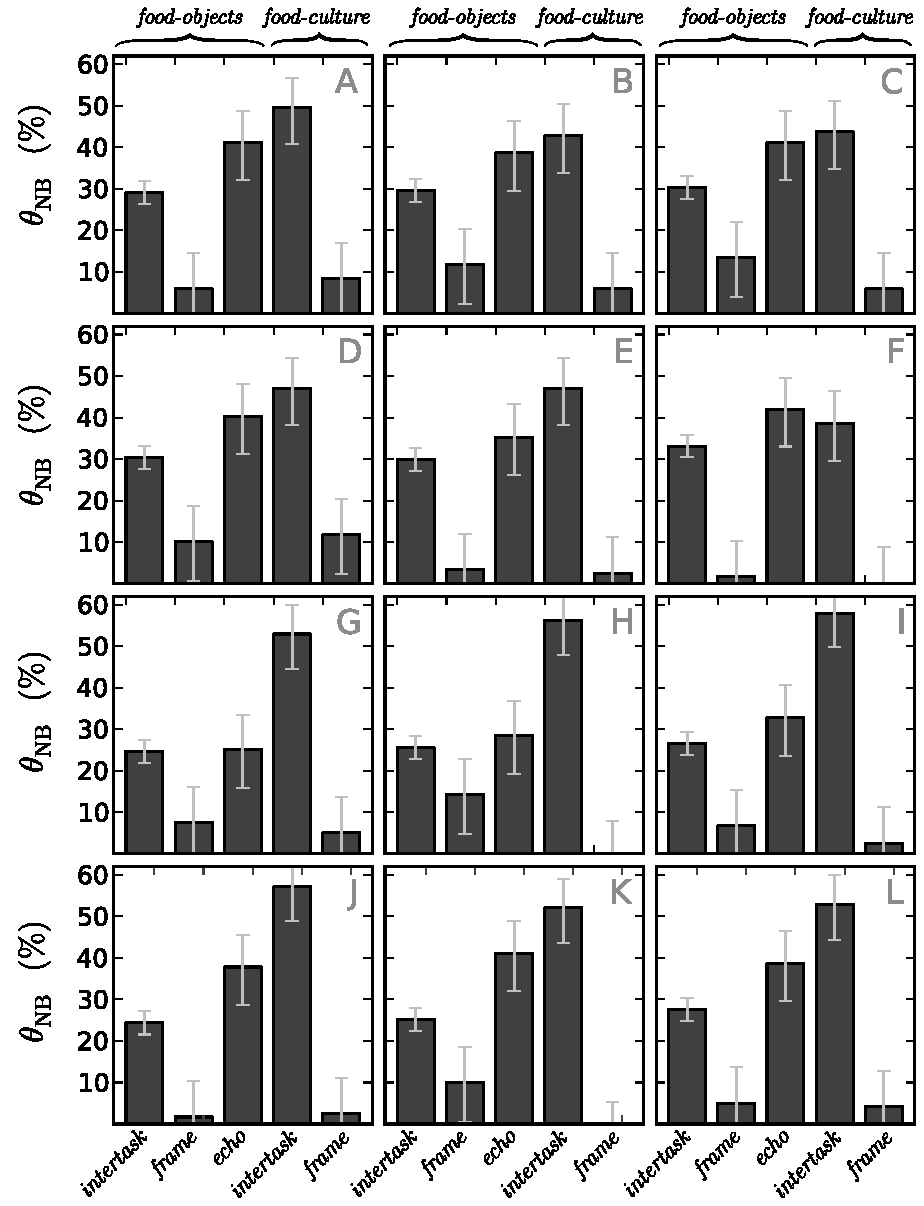
\includegraphics[scale=0.75]{figs/theta_sup.pdf}
	\label{fig:theta_sup}
	\caption{
		Figure S2: Bias induced by exposure to initial tasks and frames.
		Bias is defined to be the difference in the probability 
		distribution over workers' labels (L1-distance).  The plotted values
		give a lower bound to the L1-distance, $D_{L1}^-$, which was 
		determined from a classifier's performance in 
		distinguishing workers that had undergone different exposures.
		The bias was determined using (A-F) a na\"ive Bayes classifier, and 
		(G-L) an SVM classifier.
		In panels A through F, each plot adds an additional
		preprocessing step to those used in the previous plot; the same is 
		done for panels G through H: A,G) No 
		preprocessing; B,H) spelling correction; C,I) stopword removal; 
		D,J) lemmatization; E,K) splitting of multiple-word labels; 
		F,L) distinguishing identical labels entered in different form inputs.
	}
\end{figure}
The inequality in Eq.~\ref{l1}
asserts that a classifiers performance in predicting class membership
bounds the L1-distance between the distributions of features for the classes.
This bound is tight for the optimal classifier, and in general, the slack
depends on how the classifier is constructed.

Therefore there may exist a classifier that is 
significantly better than the one used to generate our results.  Even before
committing to a particular classifier algorithm, various decisions about
preprocessing need to be made.  For example, we chose to remove stopwords,
lemmatize, split multi-word labels, distinguish the input used to enter 
labels, and correct spelling.  All of these decisions affect the classifier
performance.  The particular classifier algorithm chosen also has a strong 
effect.

Since we did not have enough data to create a separate test set, we could not
optimize these decisions.  Doing so would lead to the inflation of the 
performance, which could then only be estimated using an independent test set.
Instead, we made principled decisions as described above.

Although we cannot optimize these decisions, it is appropriate to look at
what affect these decisions had, post-hoc.  We reproduce the plot shown in 
Fig.~\ref{fig:theta}A using different combinations of preprocessing options,
and using both the na\"ive Bayes and an SVM classifier.

Unlike the na\"ive Bayes classifier, it is necessary to tune the cost and 
gamma hyperparameters of the SVM classifier, as well as choose a kernel.
We used simulated annealing to optimize the cost and gamma settings in the
classification of $task2:food$ vs $task2:cult$.  For this reason, we expect
the bar for $task2$ in Fig.~S8G-J is likely to be an overestimate due to
overfitting on those data.

These plots show that the result shown in Fig.~\ref{fig:theta}A is 
representative, and supports the validity of the lower bounds on the 
exposures exposure effects presented in the main text, in terms of induced 
L1-distance.


\subsection*{S9: Justifications and statistical properties of classifier-based measurement of computational hysteresis}
\begin{itemize}
	\item{Relationship to L1-Distance}
	\item{Relationship to bias}
	\item{Relationship to Jenson-Shannon divergence}
	\item{Other approaches to measuring L1-distance}
	\item{Comparison to hypothesis testing using $\chi^2$}
\end{itemize}



\end{document}

